\newpage{}
\section{Eje Y}
	\subsection{Material necesario}
		\begin{itemize}
			\item Madera.
			\item Piezas Y Barend.
			\item Piezas BeltClip
			\item Base Caliente.
			\item 4x Muelles 30mm.
			\item 16x arandelas M3.
			\item 13x tuercas M3.
			\item 8x tornillos M3x30.
			\item 5x tornillos M3x15.
			\item 4x clemas.
		\end{itemize}
		\begin{figure}[!htp]
			\centering
			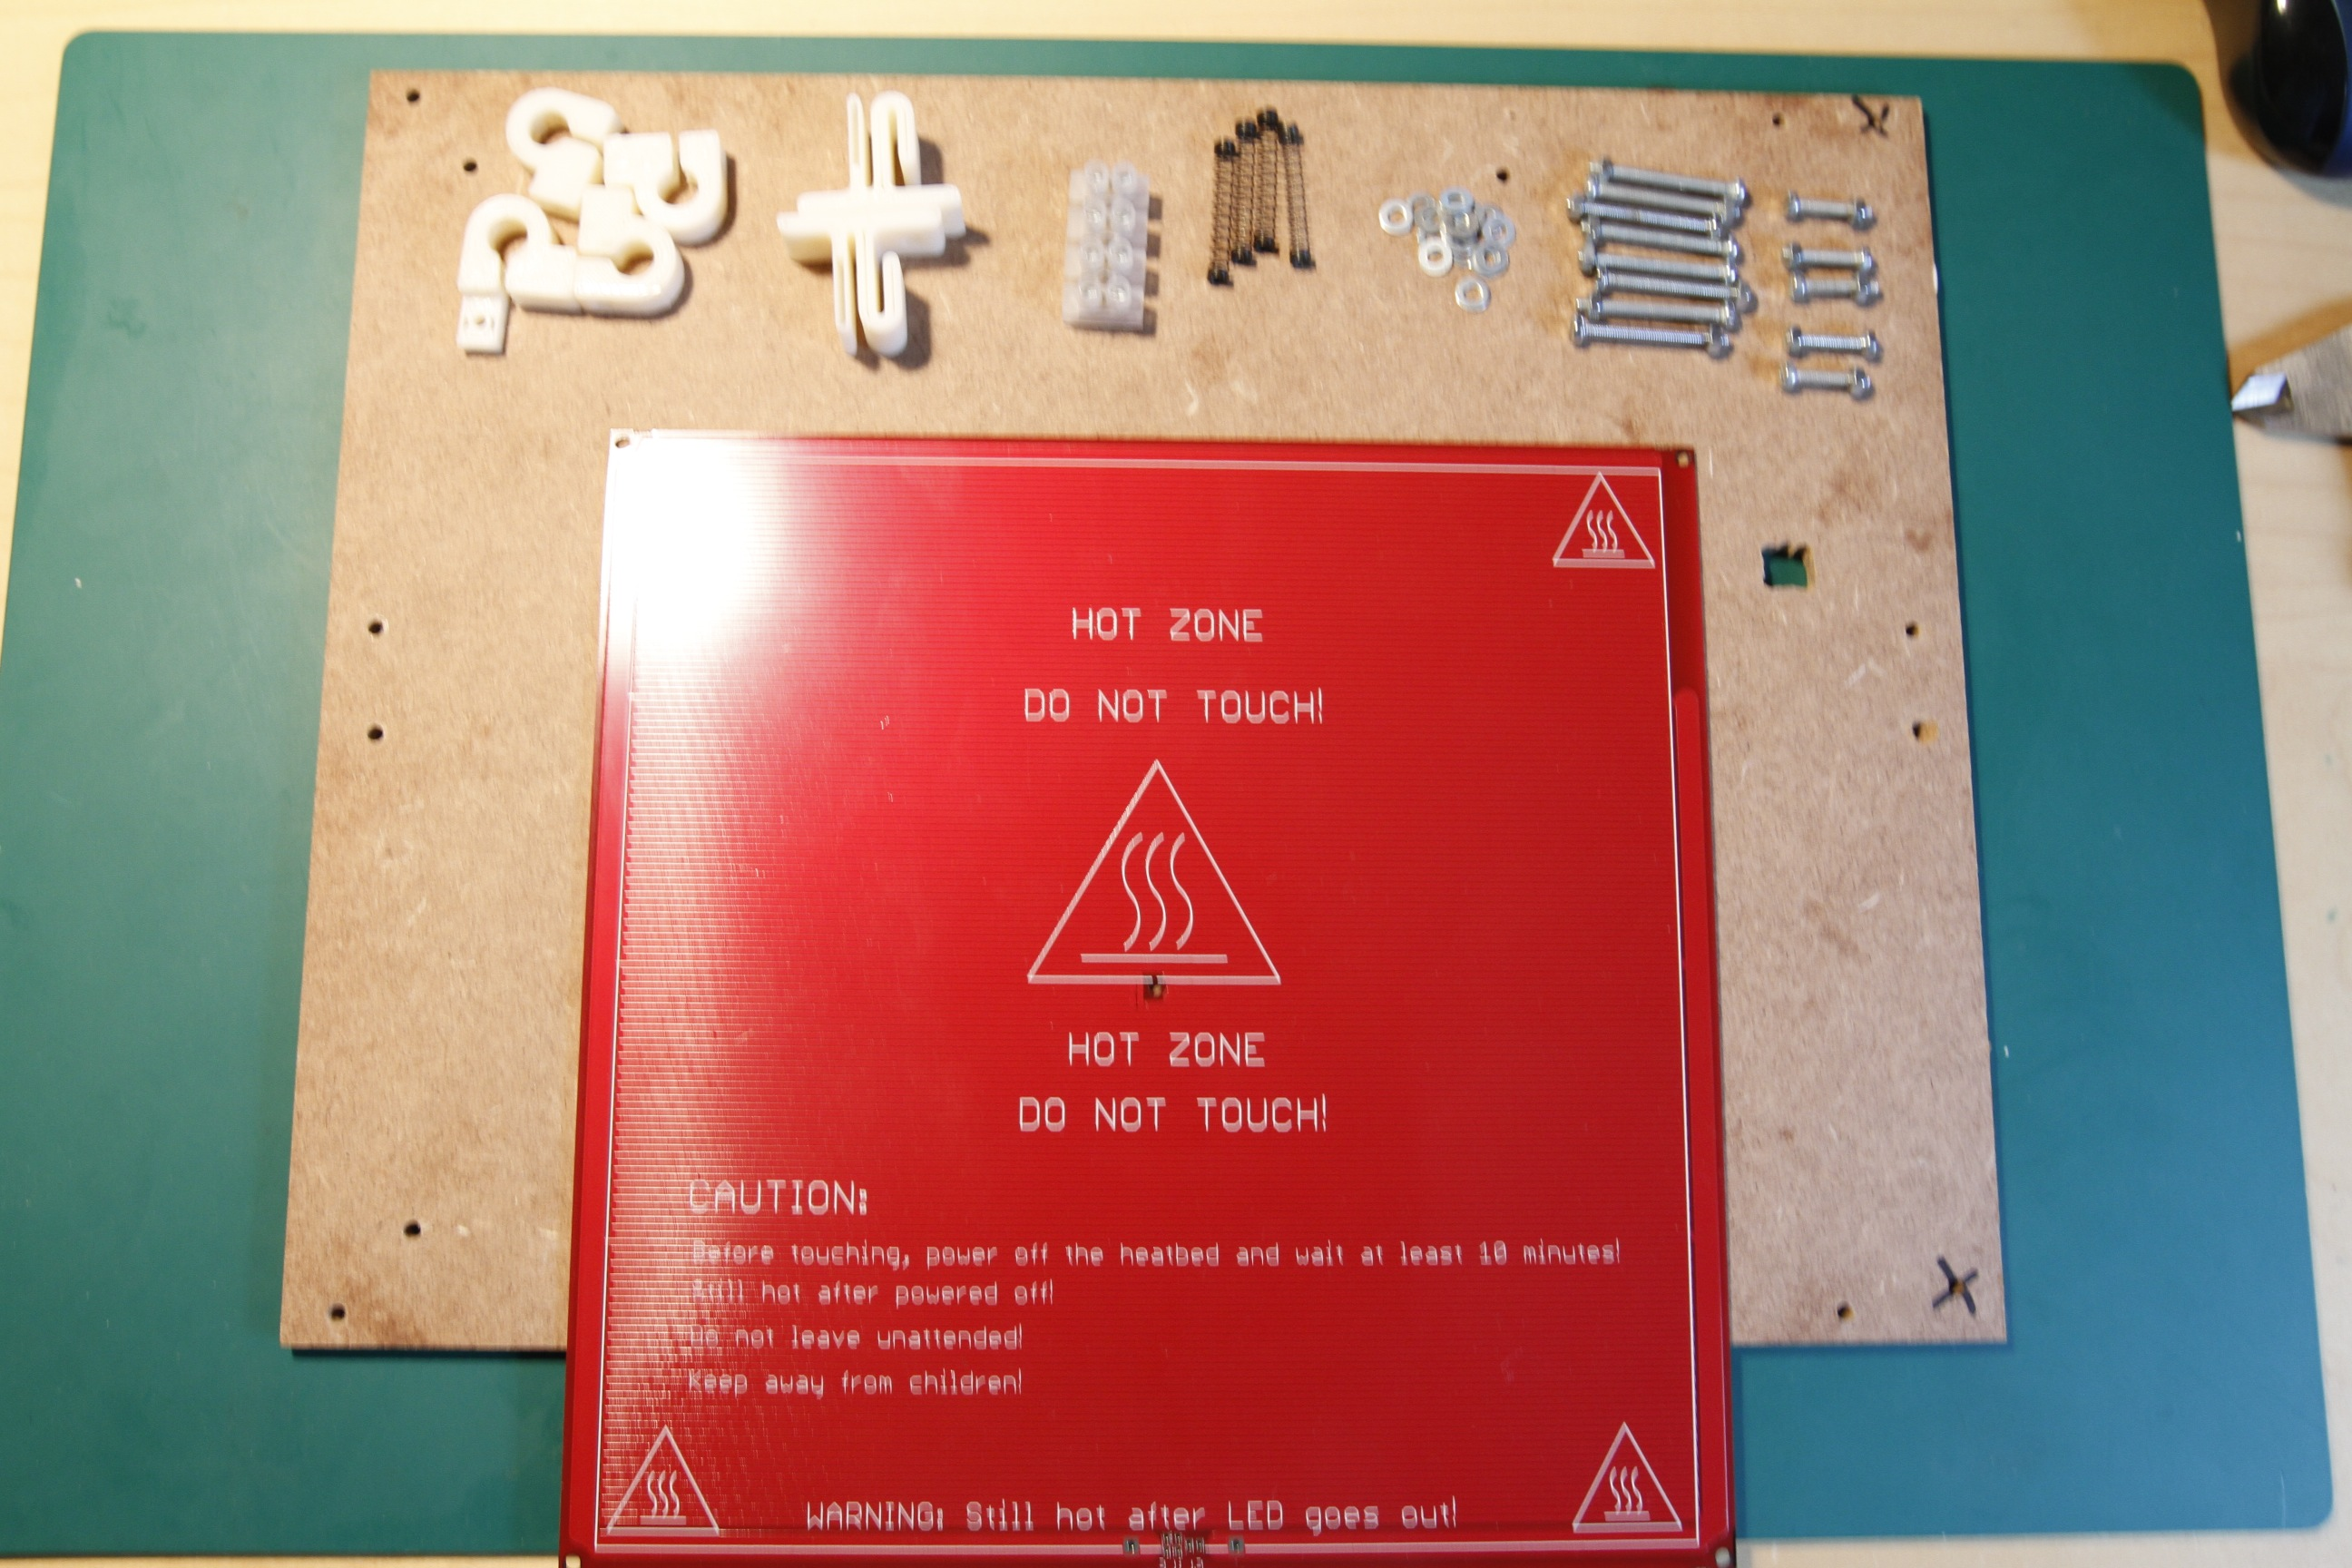
\includegraphics[width=0.7\textwidth]{../../Fotos/33.jpg}
			\caption{Material necesario}
		\end{figure}
		\newpage{}
	\subsection{Herramienta necesaria}
		\begin{itemize}
			\item Alicates de punta fina.
			\item Destornillador.
		\end{itemize}
		\begin{figure}[!htp]
			\centering
			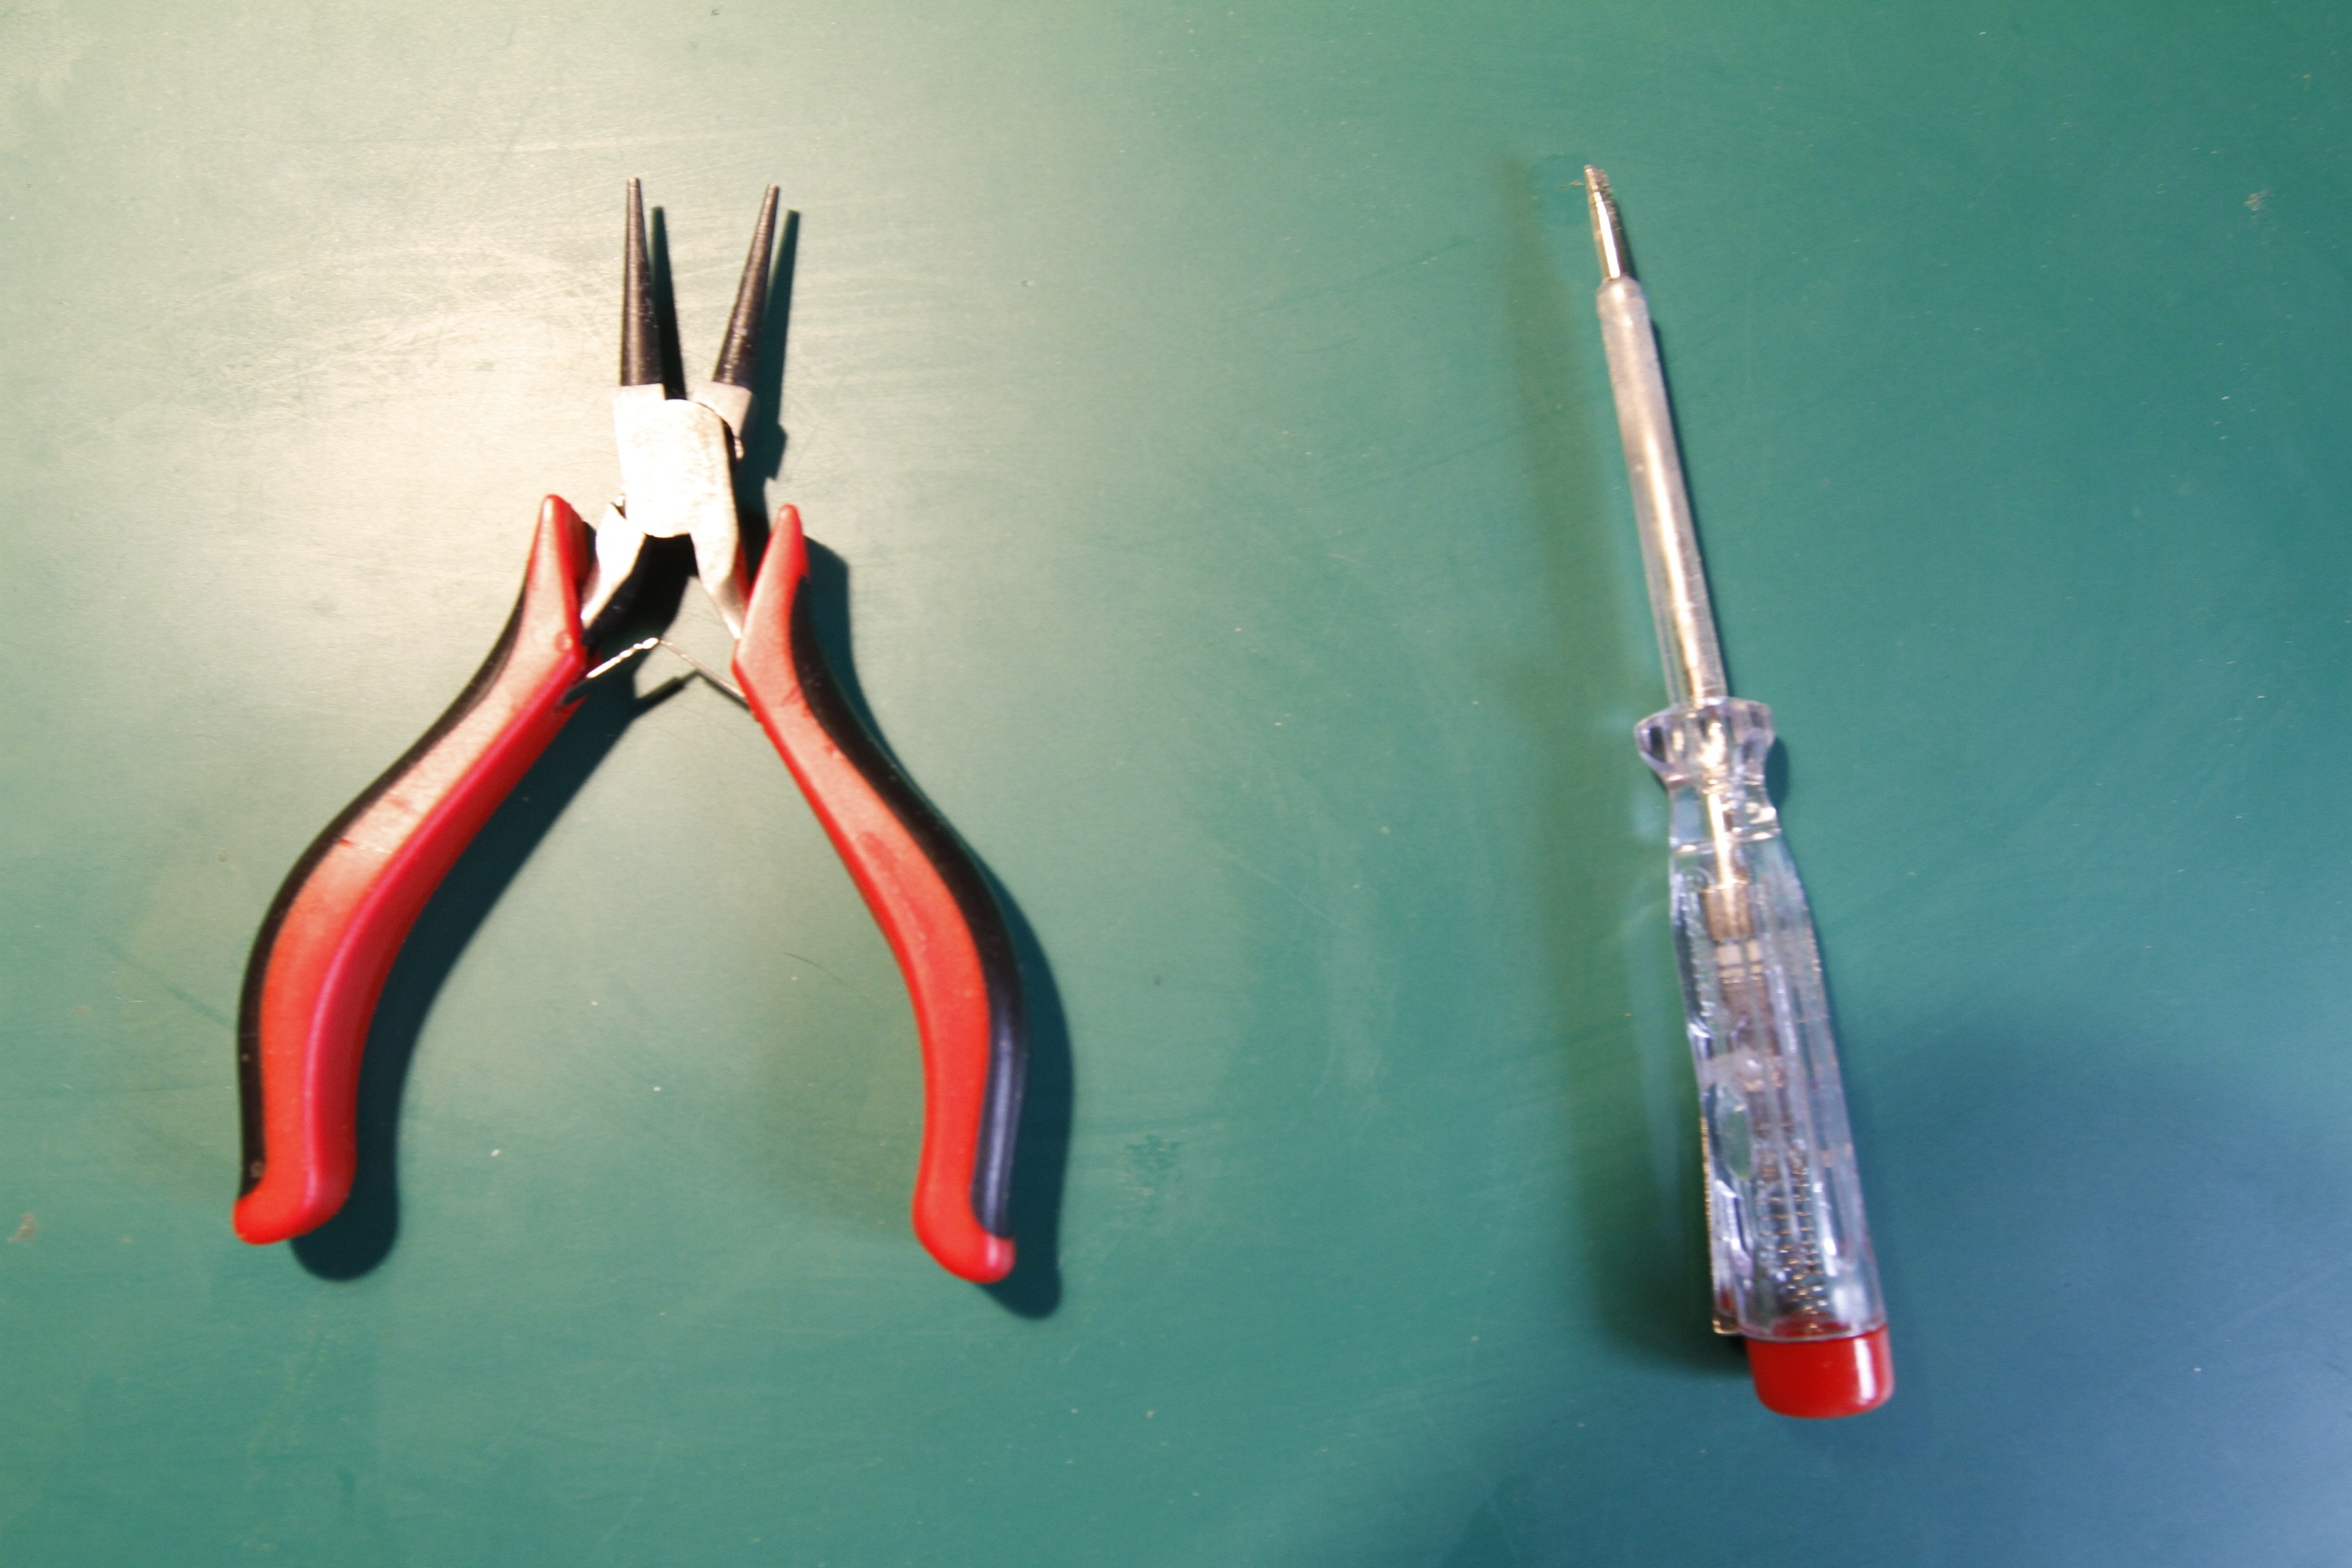
\includegraphics[width=0.7\textwidth]{../../Fotos/34.jpg}
			\caption{Herramienta necesaria}
		\end{figure}
		\newpage{}
	\subsection{Operativa}
	Preparamos el cable grueso de 10 cm, pelando ambas puntas del cable. A continuación, introducimos parte de los hilillos de cada uno de los cables por los dos agujeros de la base caliente. Hacemos una bola con los hilos que sobresalen por debajo y cortamos los sobrantes por arriba. Despues, soldamos con estaño ambos cables por debajo y por arriba de la base caliente. En la otra punta del cable, estañamos ambas terminaciones, que irán después a una clema en la Sanguinololu.
	\begin{figure}[H]
	    \centering
	    \begin{subfigure}[b]{0.4\textwidth}
	        \centering
	        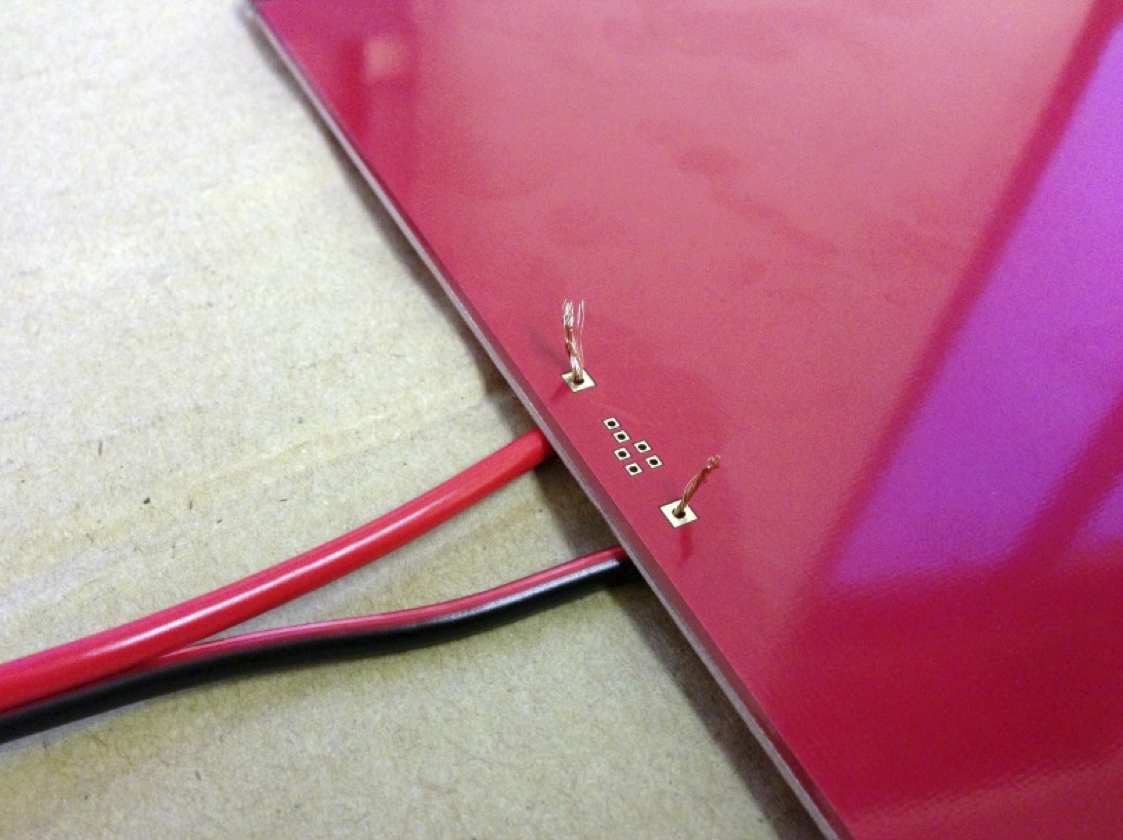
\includegraphics[width=\textwidth]{../../Fotos/36b.jpg}
	    \end{subfigure}
	    \begin{subfigure}[b]{0.4\textwidth}
	       \centering
	       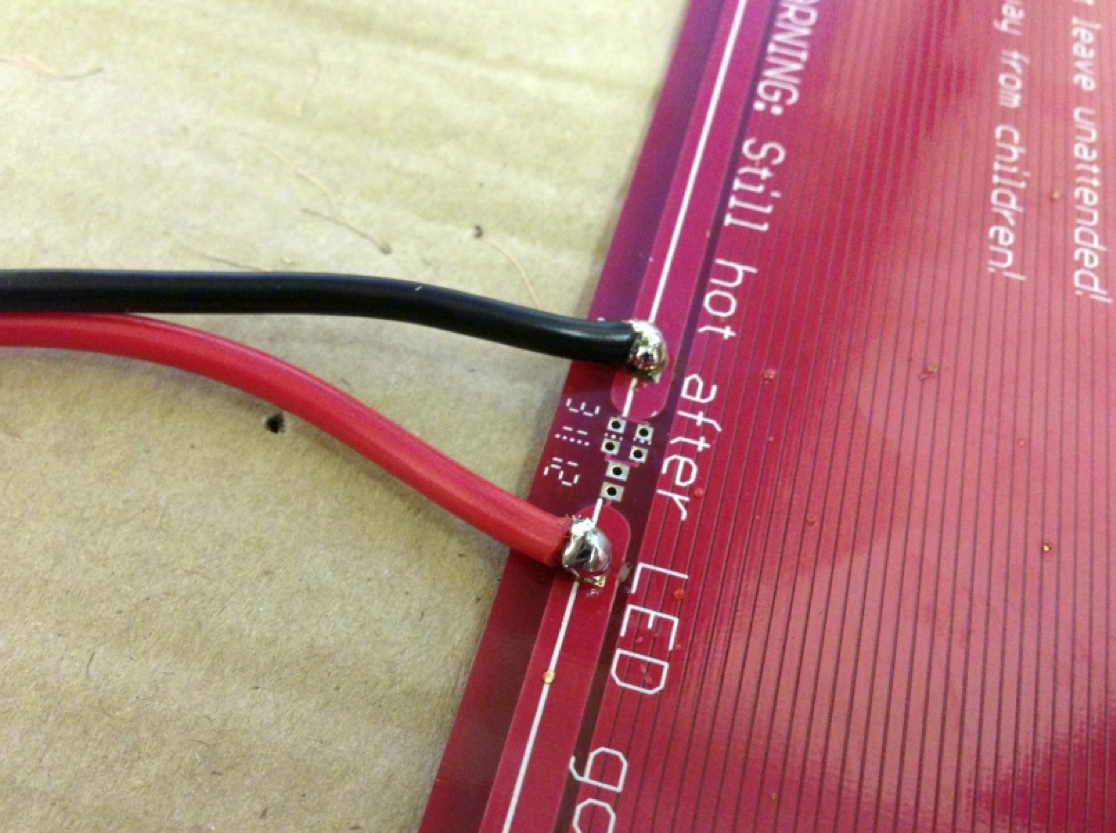
\includegraphics[width=\textwidth]{../../Fotos/36c.jpg}
	       
	    \end{subfigure}
	    \caption{Soldando Cables a la base caliente}\label{fig:1.y}
	\end{figure}
	Después soldaremos un termistor a un cable con conector de dos agujeros. Es recomendable utilizar algo de termoretractil. Por ultimo colocamos el termistor como aparece en la imagen, y lo sujetamos todo con kapton.
	\begin{figure}[H]
	    \centering
	    \begin{subfigure}[b]{0.4\textwidth}
	        \centering
	        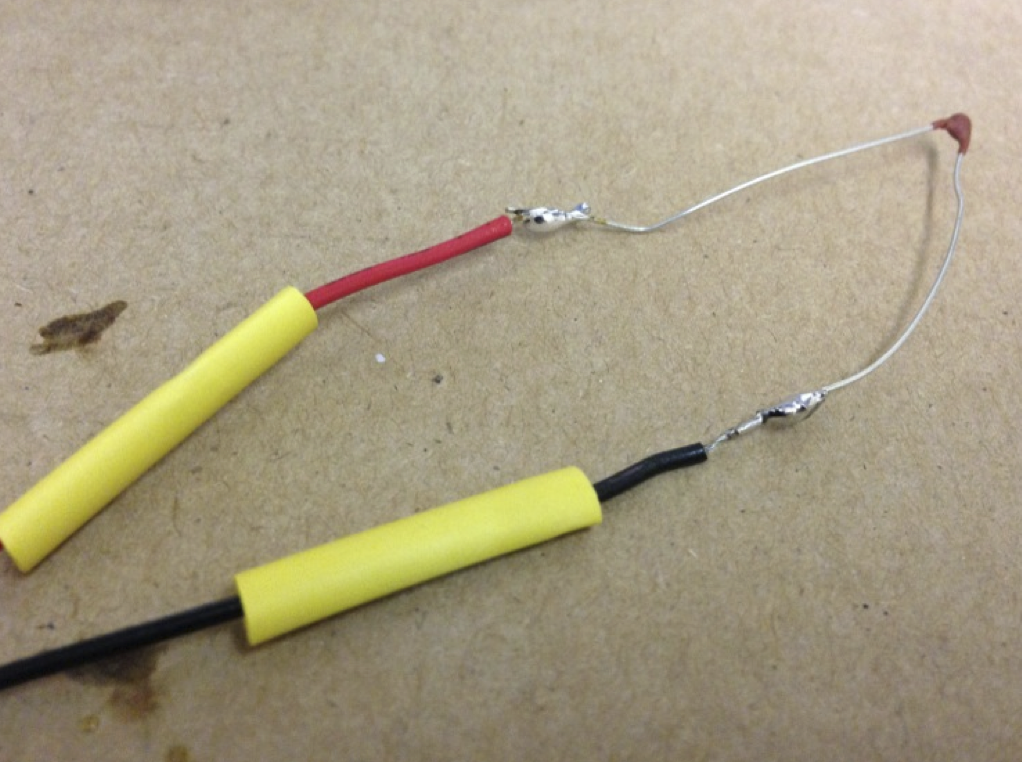
\includegraphics[width=\textwidth]{../../Fotos/36d.jpg}
	    \end{subfigure}
	    \begin{subfigure}[b]{0.4\textwidth}
	       \centering
	       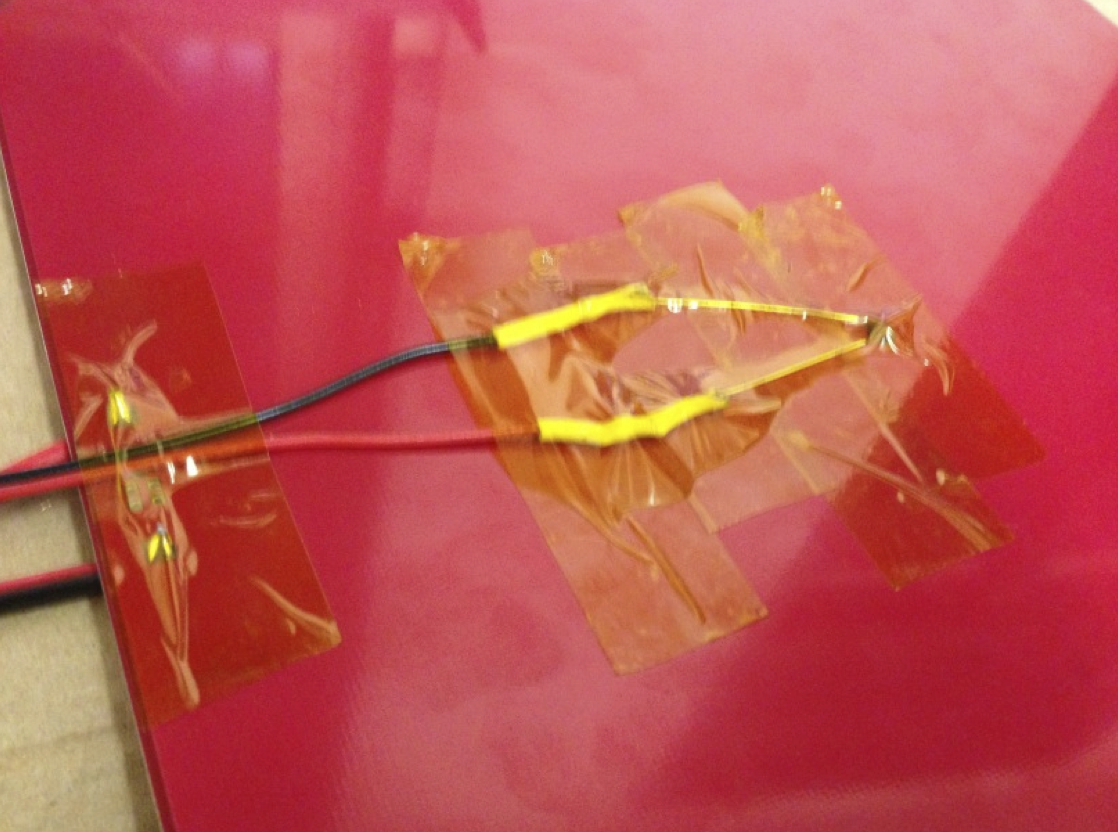
\includegraphics[width=\textwidth]{../../Fotos/36e.jpg}
	       
	    \end{subfigure}
	    \caption{Soldando Termistor}\label{fig:2.y}
	\end{figure}
	Colocaremos lo primero de todo la base caliente en la madera perforada.Para ello colocaremos las conexiones lo más cerca del cuadrado perforado. Fijaremos la placa a la madera mediante tornillos y muelles, (Ver figura ~\ref{fig:colocacion.heatbed})\\

		  \begin{figure}[H]
		        \centering
		        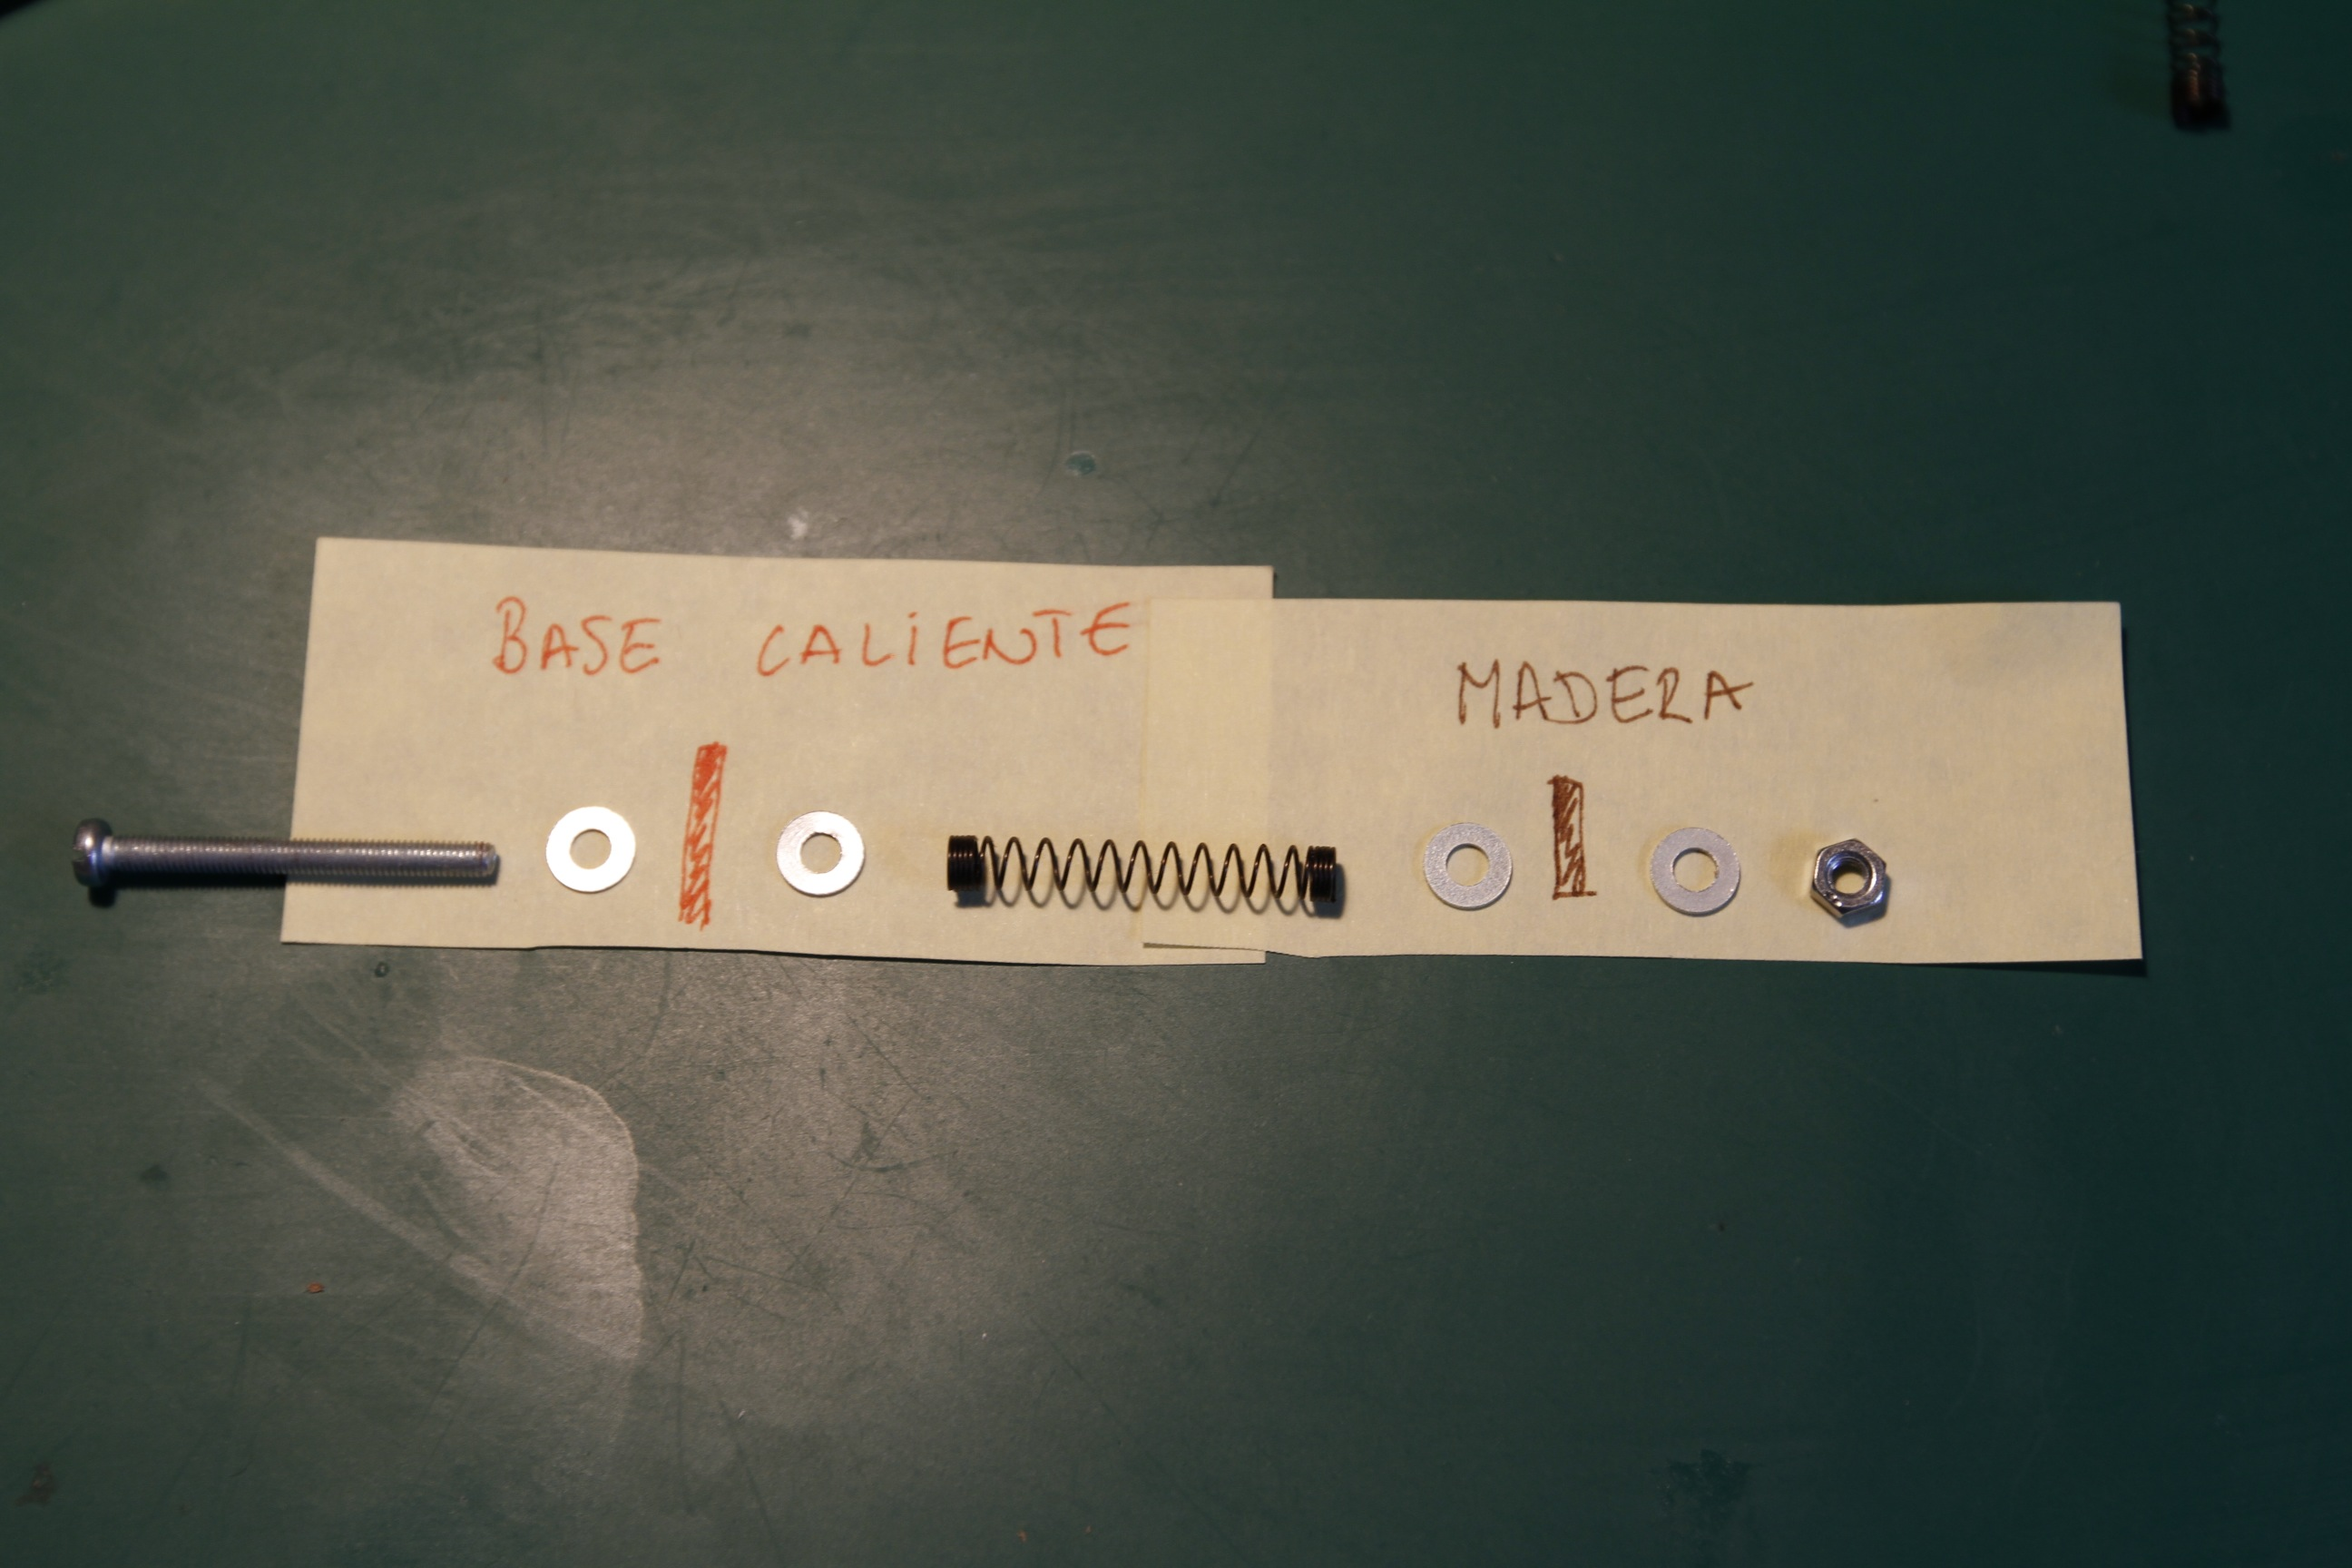
\includegraphics[width=0.7\textwidth]{../../Fotos/35.jpg}
		        \caption{Vista explosionada.}
		        \label{fig:colocacion.heatbed}
		    \end{figure}

		    \begin{figure}[H]
		       \centering
		       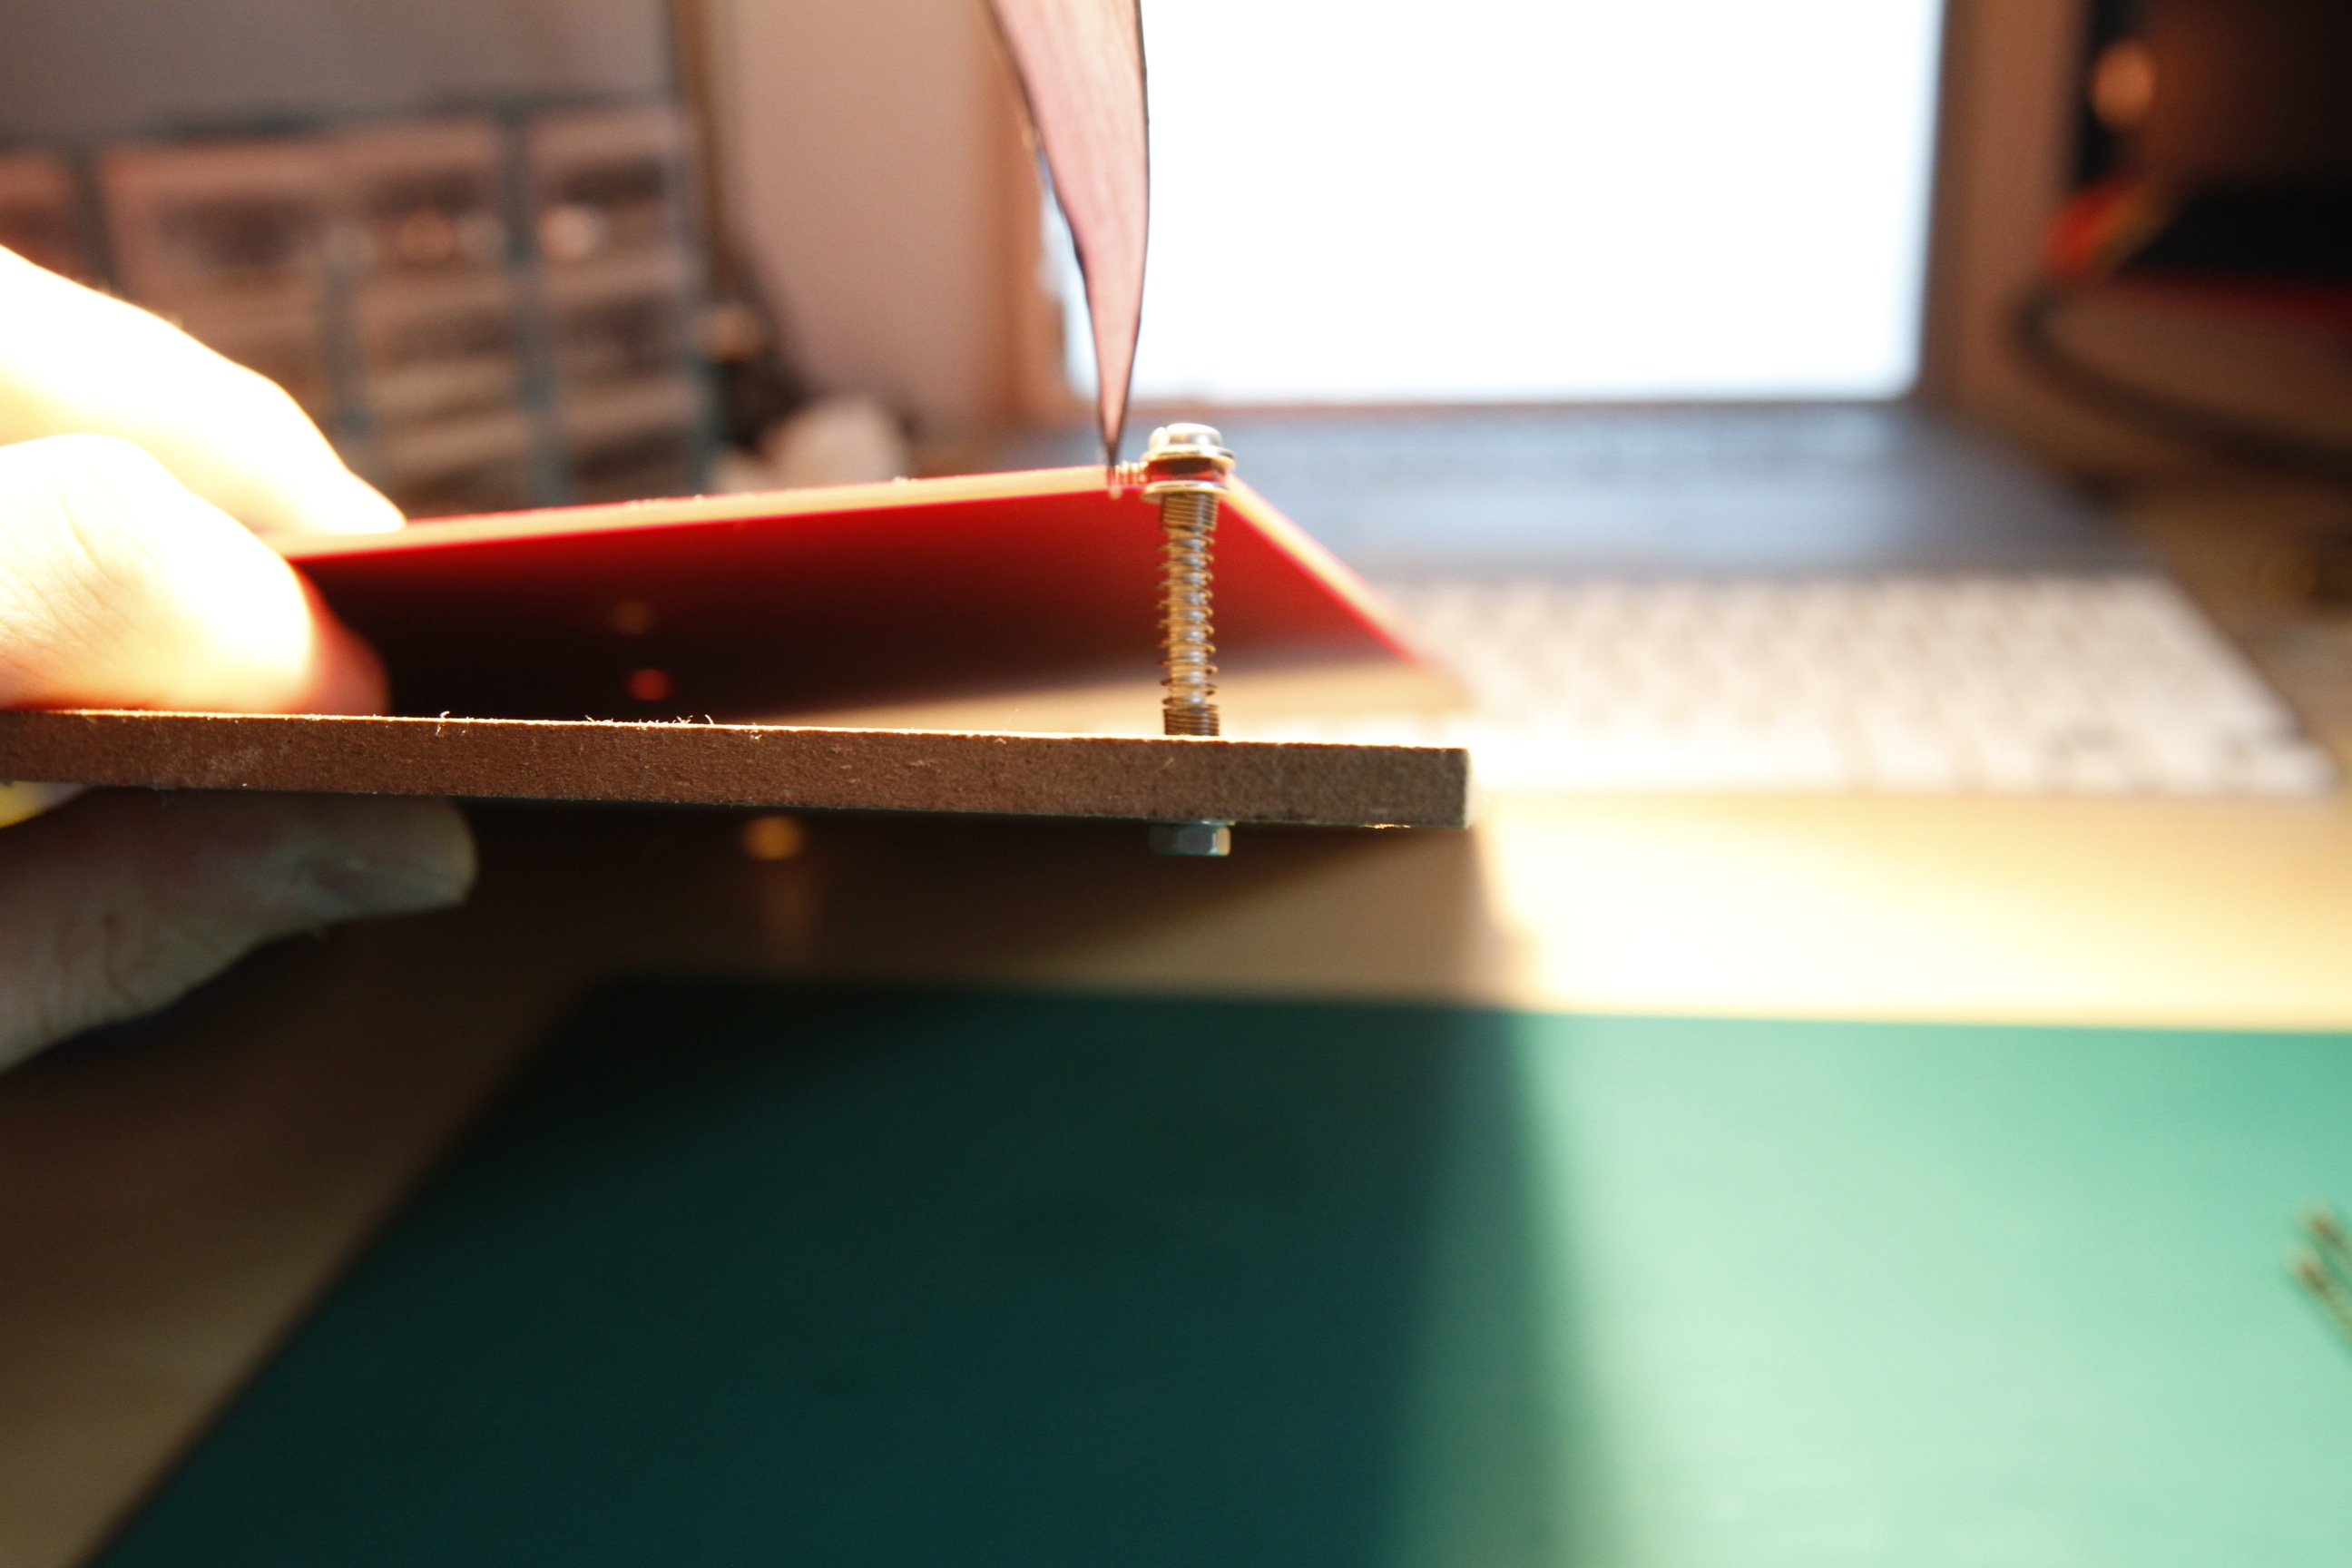
\includegraphics[width=0.8\textwidth]{../../Fotos/36.jpg}
		       \caption{Colocación final.}
		       \label{fig:colocado.heatbed}
		    \end{figure}
		    \newpage{}
	La mejor manera de colocar los tornillos es, primero los de una diagonal y a continuación los otros, en este paso no es necesario apretar los tornillos ni nivelar la base. El aspecto final lo podemos ver en la figura ~\ref{fig:montada.heatbed}. Es muy importante fijarse en la colocación de las letras con respecto a la madera.\\
		\begin{figure}[H]
			\centering
			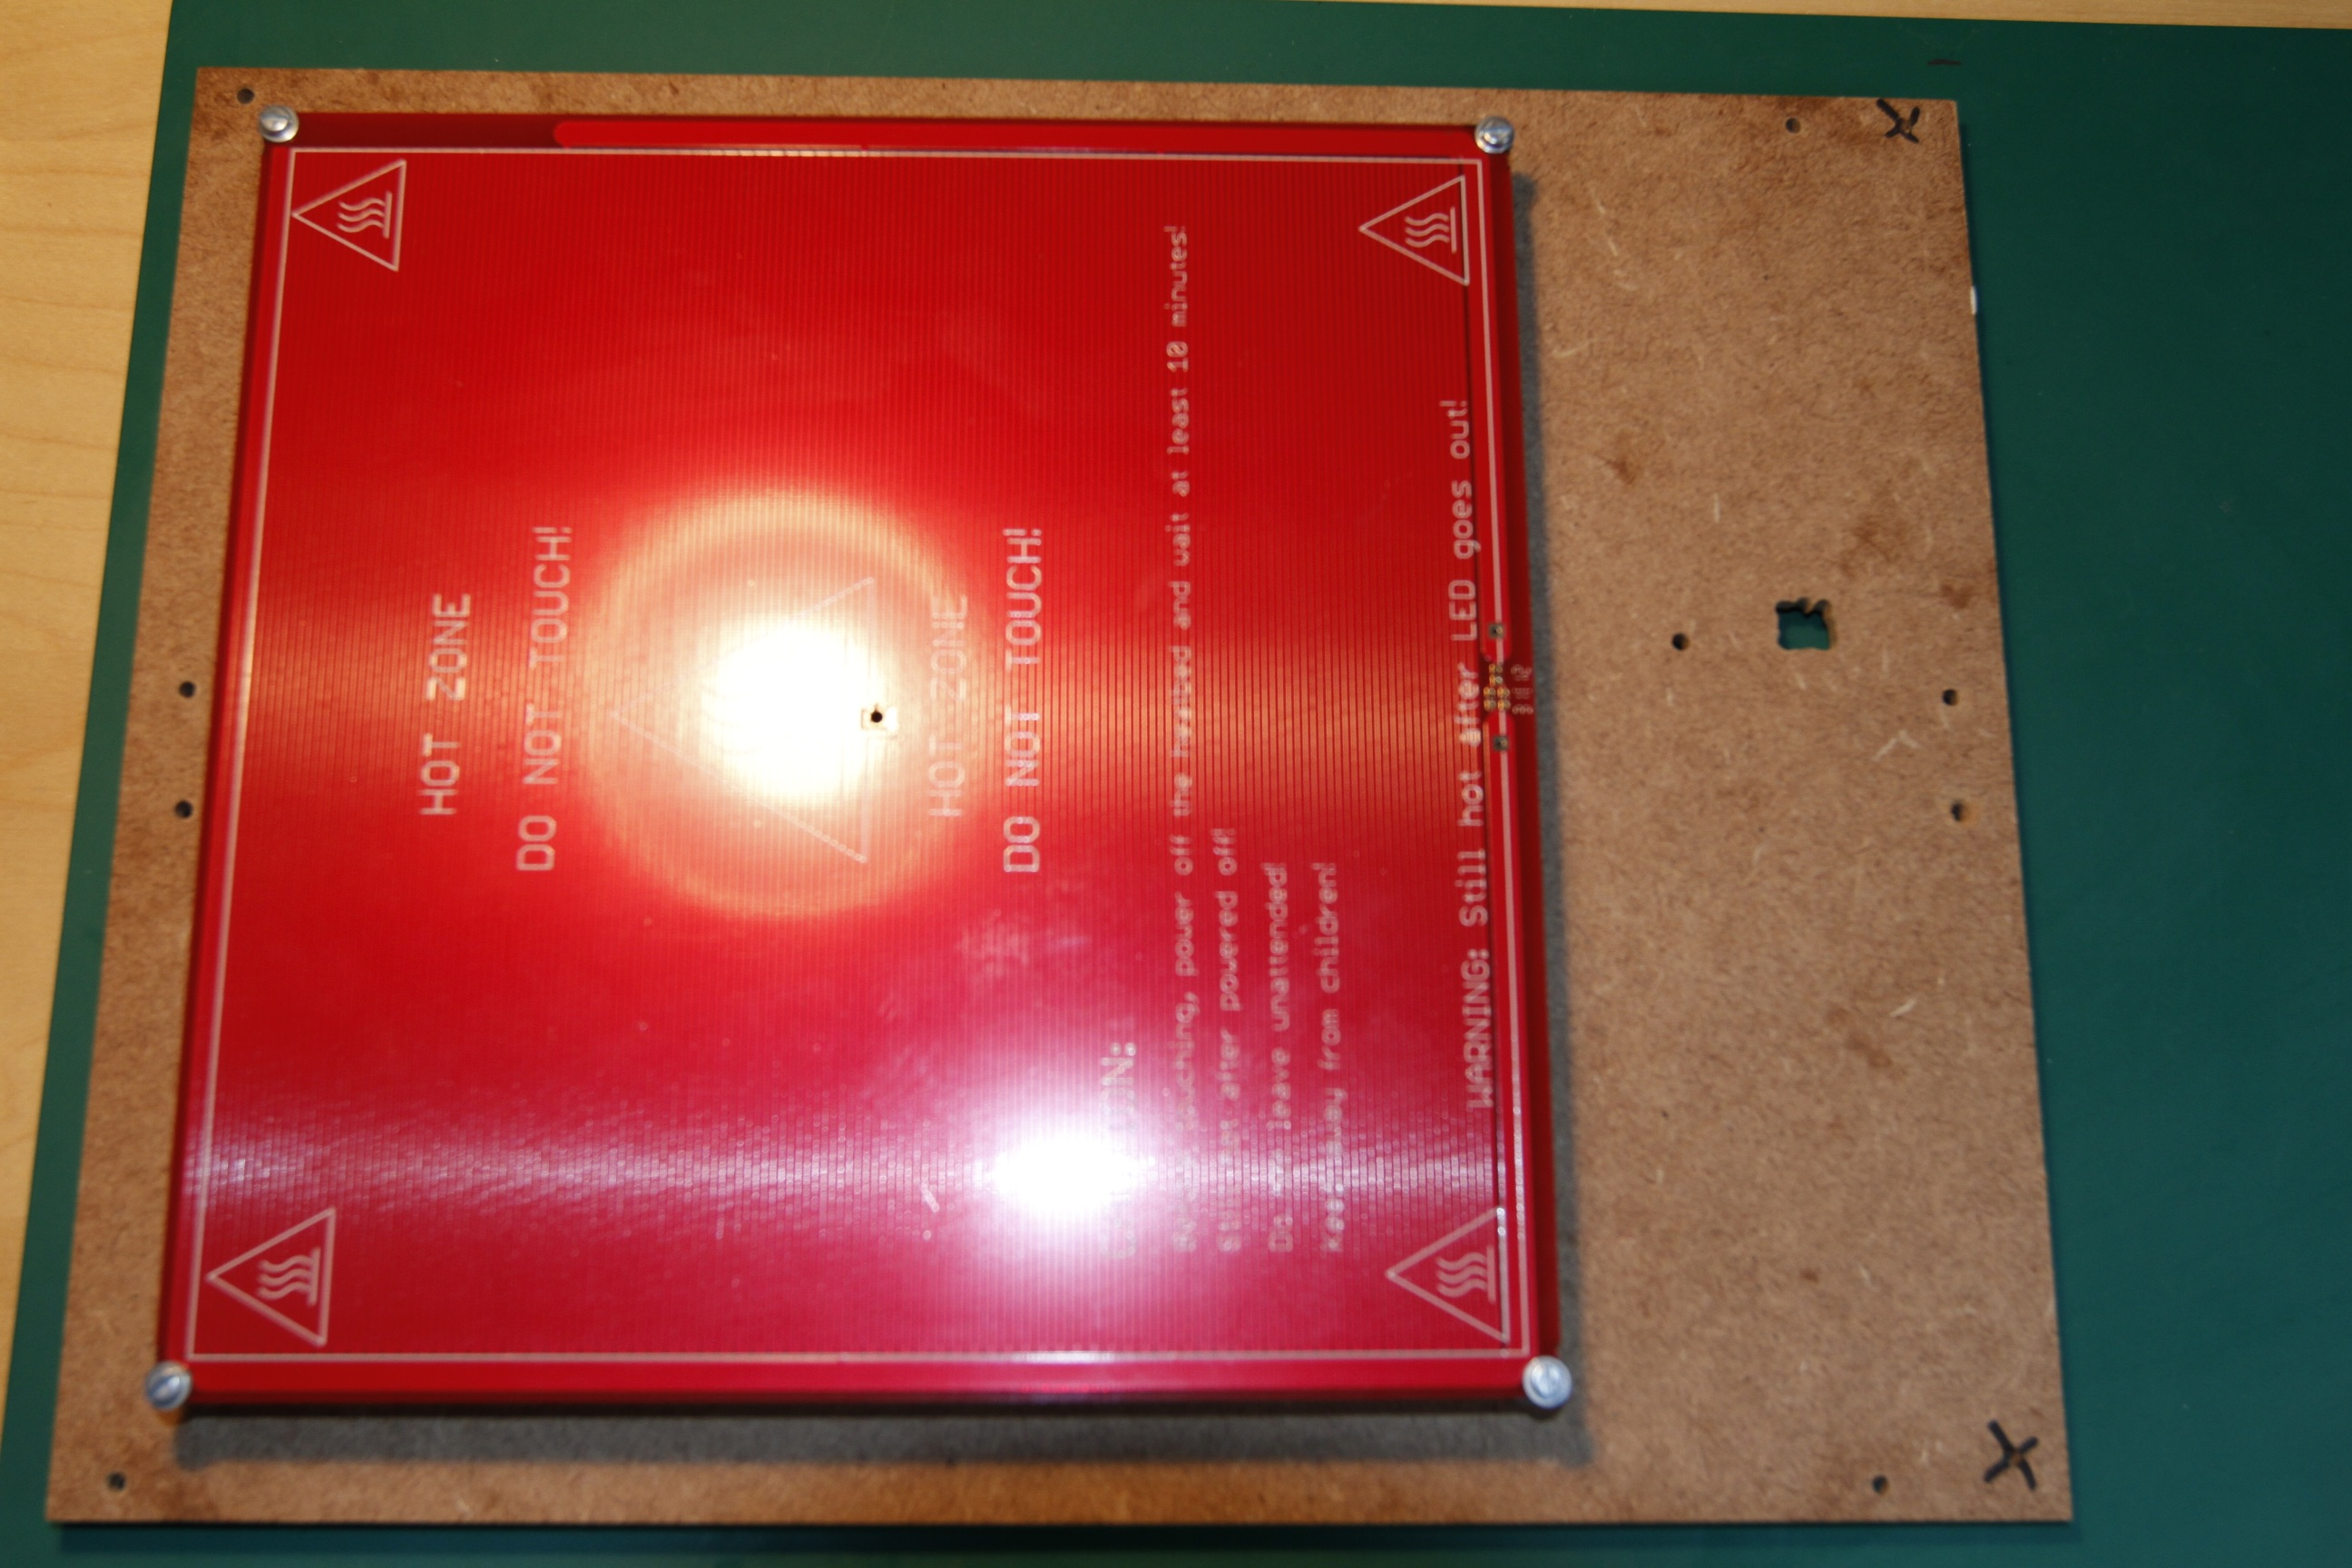
\includegraphics[width=0.7\textwidth]{../../Fotos/37.jpg}
			\caption{Limando drivers de potencia}
			\label{fig:montada.heatbed}
		\end{figure}
	Lo siguiente es colocar las piezas impresas que sujetaran las barras lisas. Una de las piezas tiene un saliente con un taladro, para colocar un tornillo y activar el endstop del eje Y, la colocación de esta pieza debe ser la superior izquierda, si colocamos la tabla como en la figura ~\ref{fig:montada.heatbed}.\\
		\begin{figure}[H]
		    \centering
		    \begin{subfigure}[b]{0.4\textwidth}
		        \centering
		        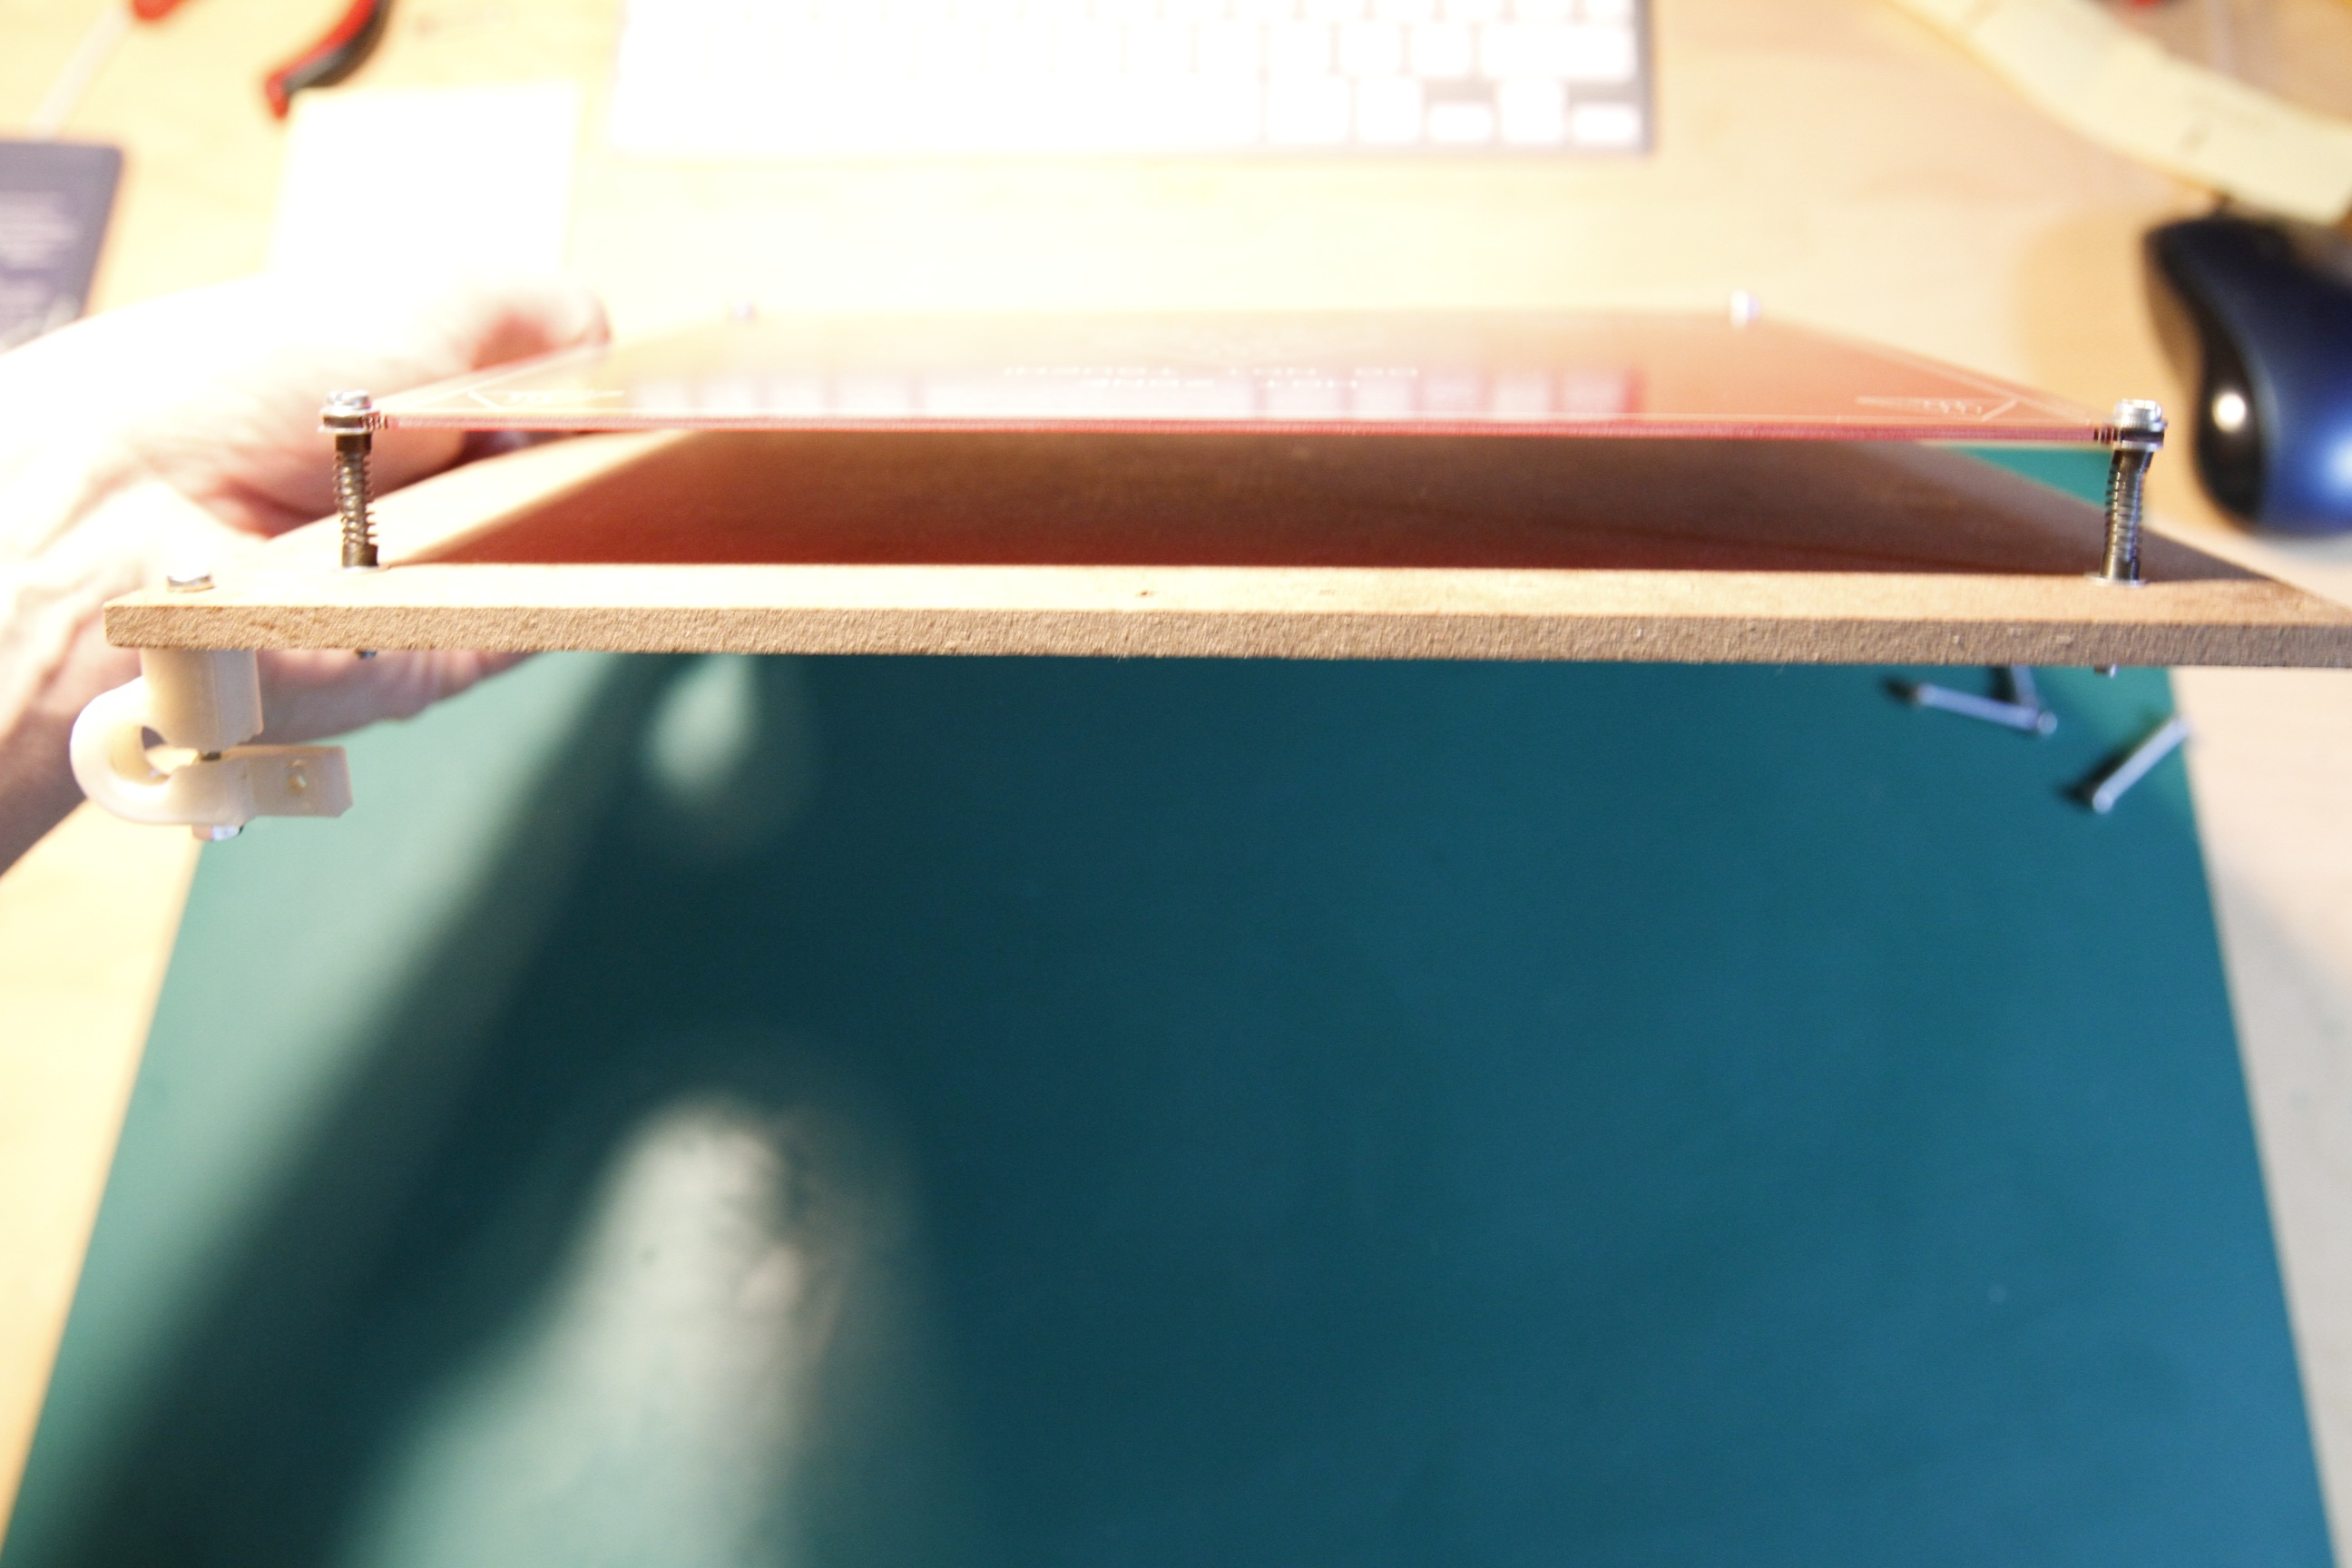
\includegraphics[width=\textwidth]{../../Fotos/39.jpg}
		        \caption{Vista de frente}
		        \label{fig:barend.frente}
		    \end{subfigure}
		    \begin{subfigure}[b]{0.4\textwidth}
		       \centering
		       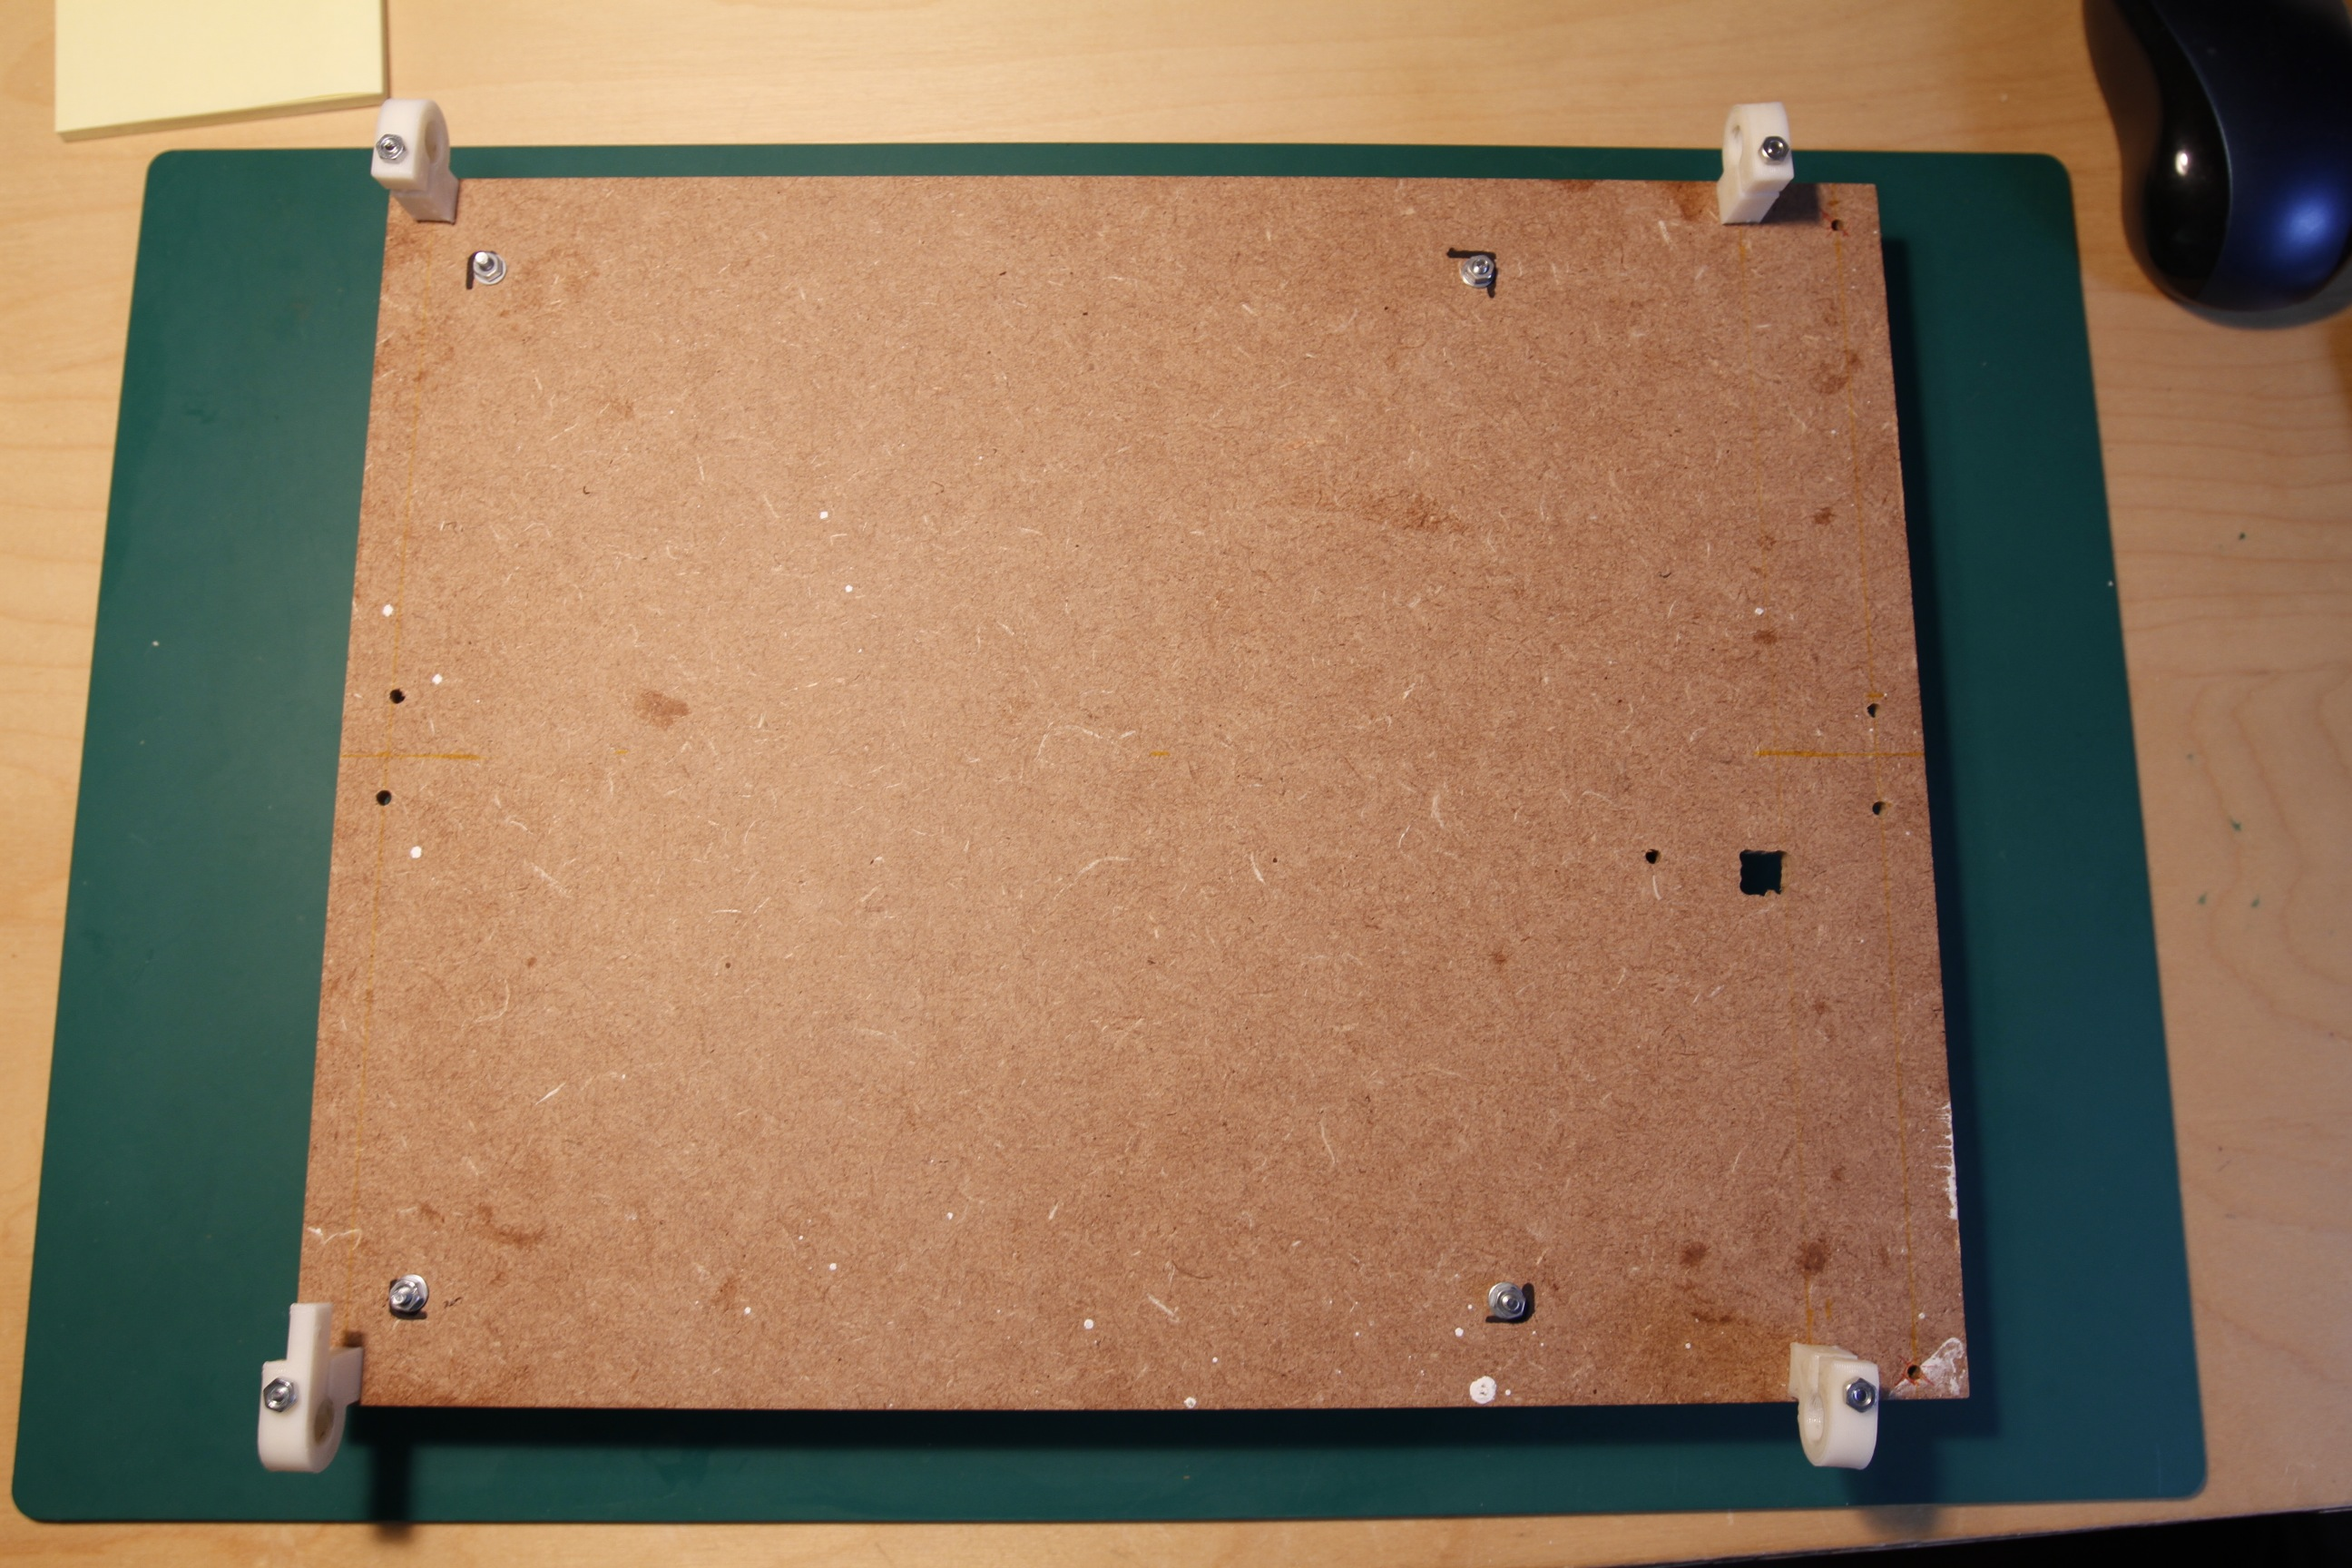
\includegraphics[width=\textwidth]{../../Fotos/40.jpg}
		       \caption{Parte inferior}
		       \label{fig:barend.inferior}
		    \end{subfigure}
		    \caption{Colocación de Y bar-end}\label{fig:barend}
		\end{figure}
	A continuación, colocaremos los soportes para poder poner la correa tensora, la posición es indistinta, lo importante es que una vez colocada la correa quede justo en el medio de la tabla. (Ver figura ~\ref{fig:beltclip}). Por útlimo colocaremos la clema en el único taladro que nos queda, cerca del cuadrado perforado, en esta clema irán los cables de alimentación de la heatbed y del termistor (Ver figura ~\ref{fig:clema}).\\
		\begin{figure}[H]
			\centering
			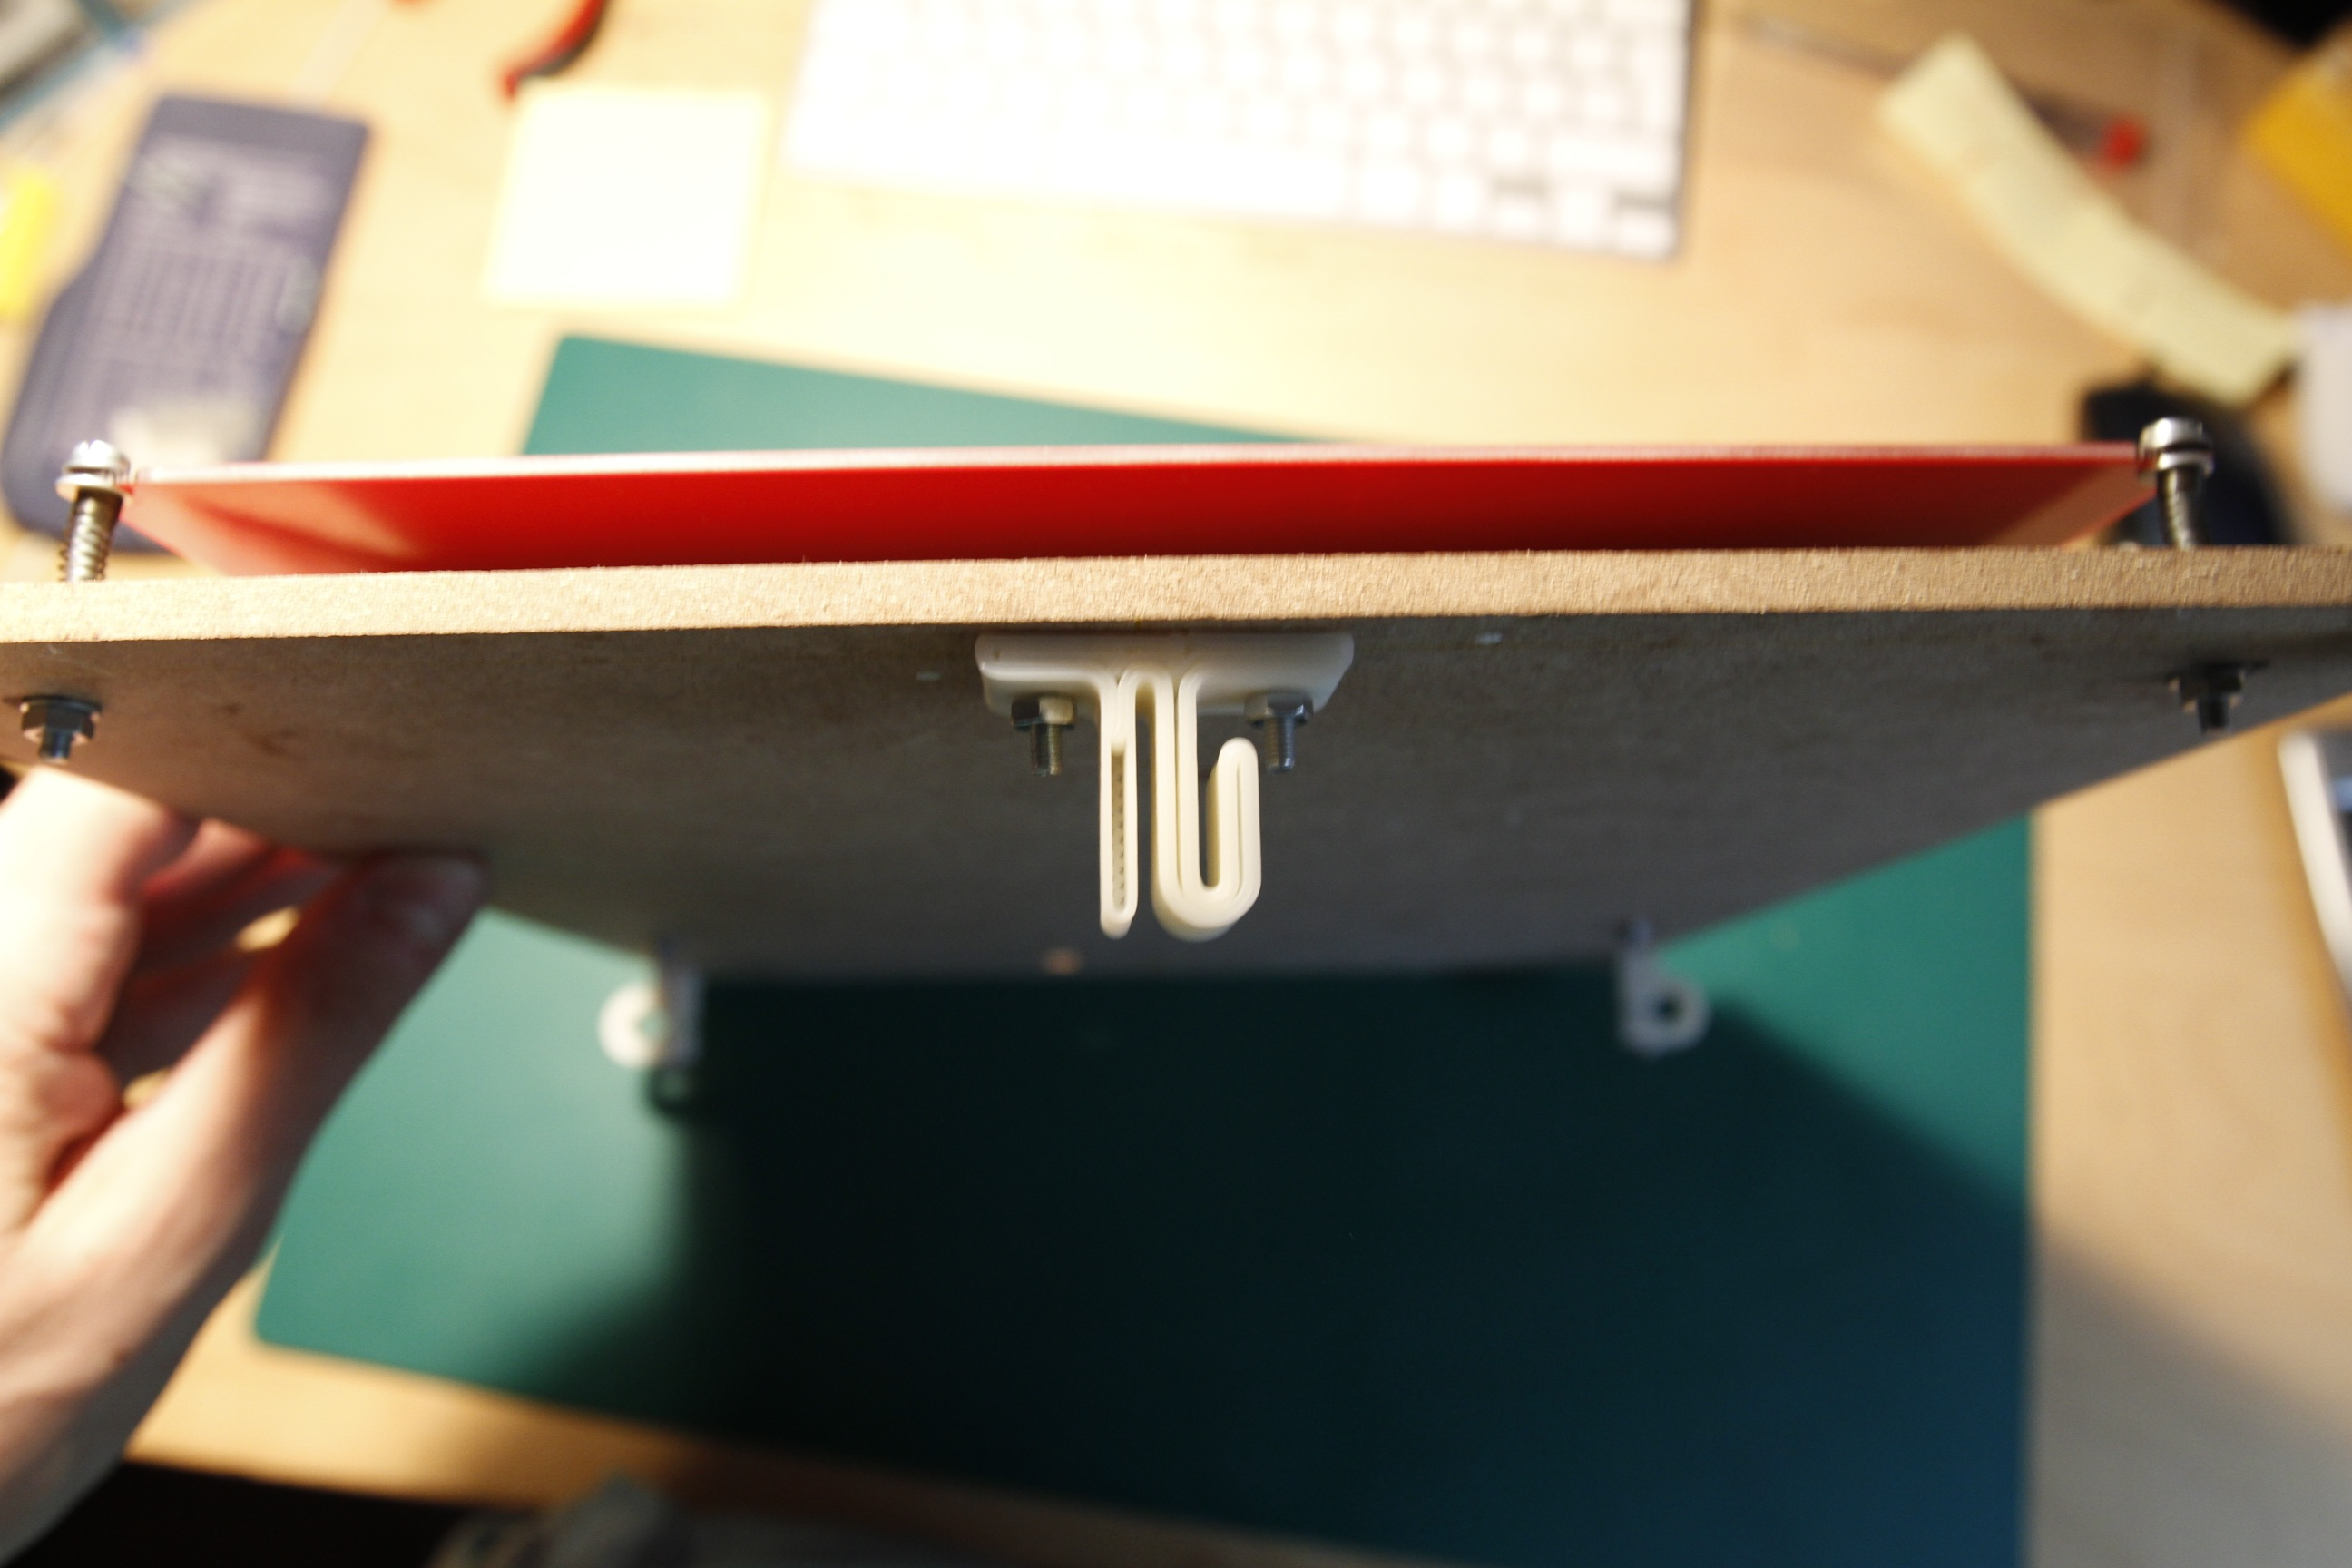
\includegraphics[width=0.7\textwidth]{../../Fotos/41.jpg}
			\caption{Posición de la pieza Beltclip}
			\label{fig:beltclip}
		\end{figure}
		\begin{figure}[H]
			\centering
			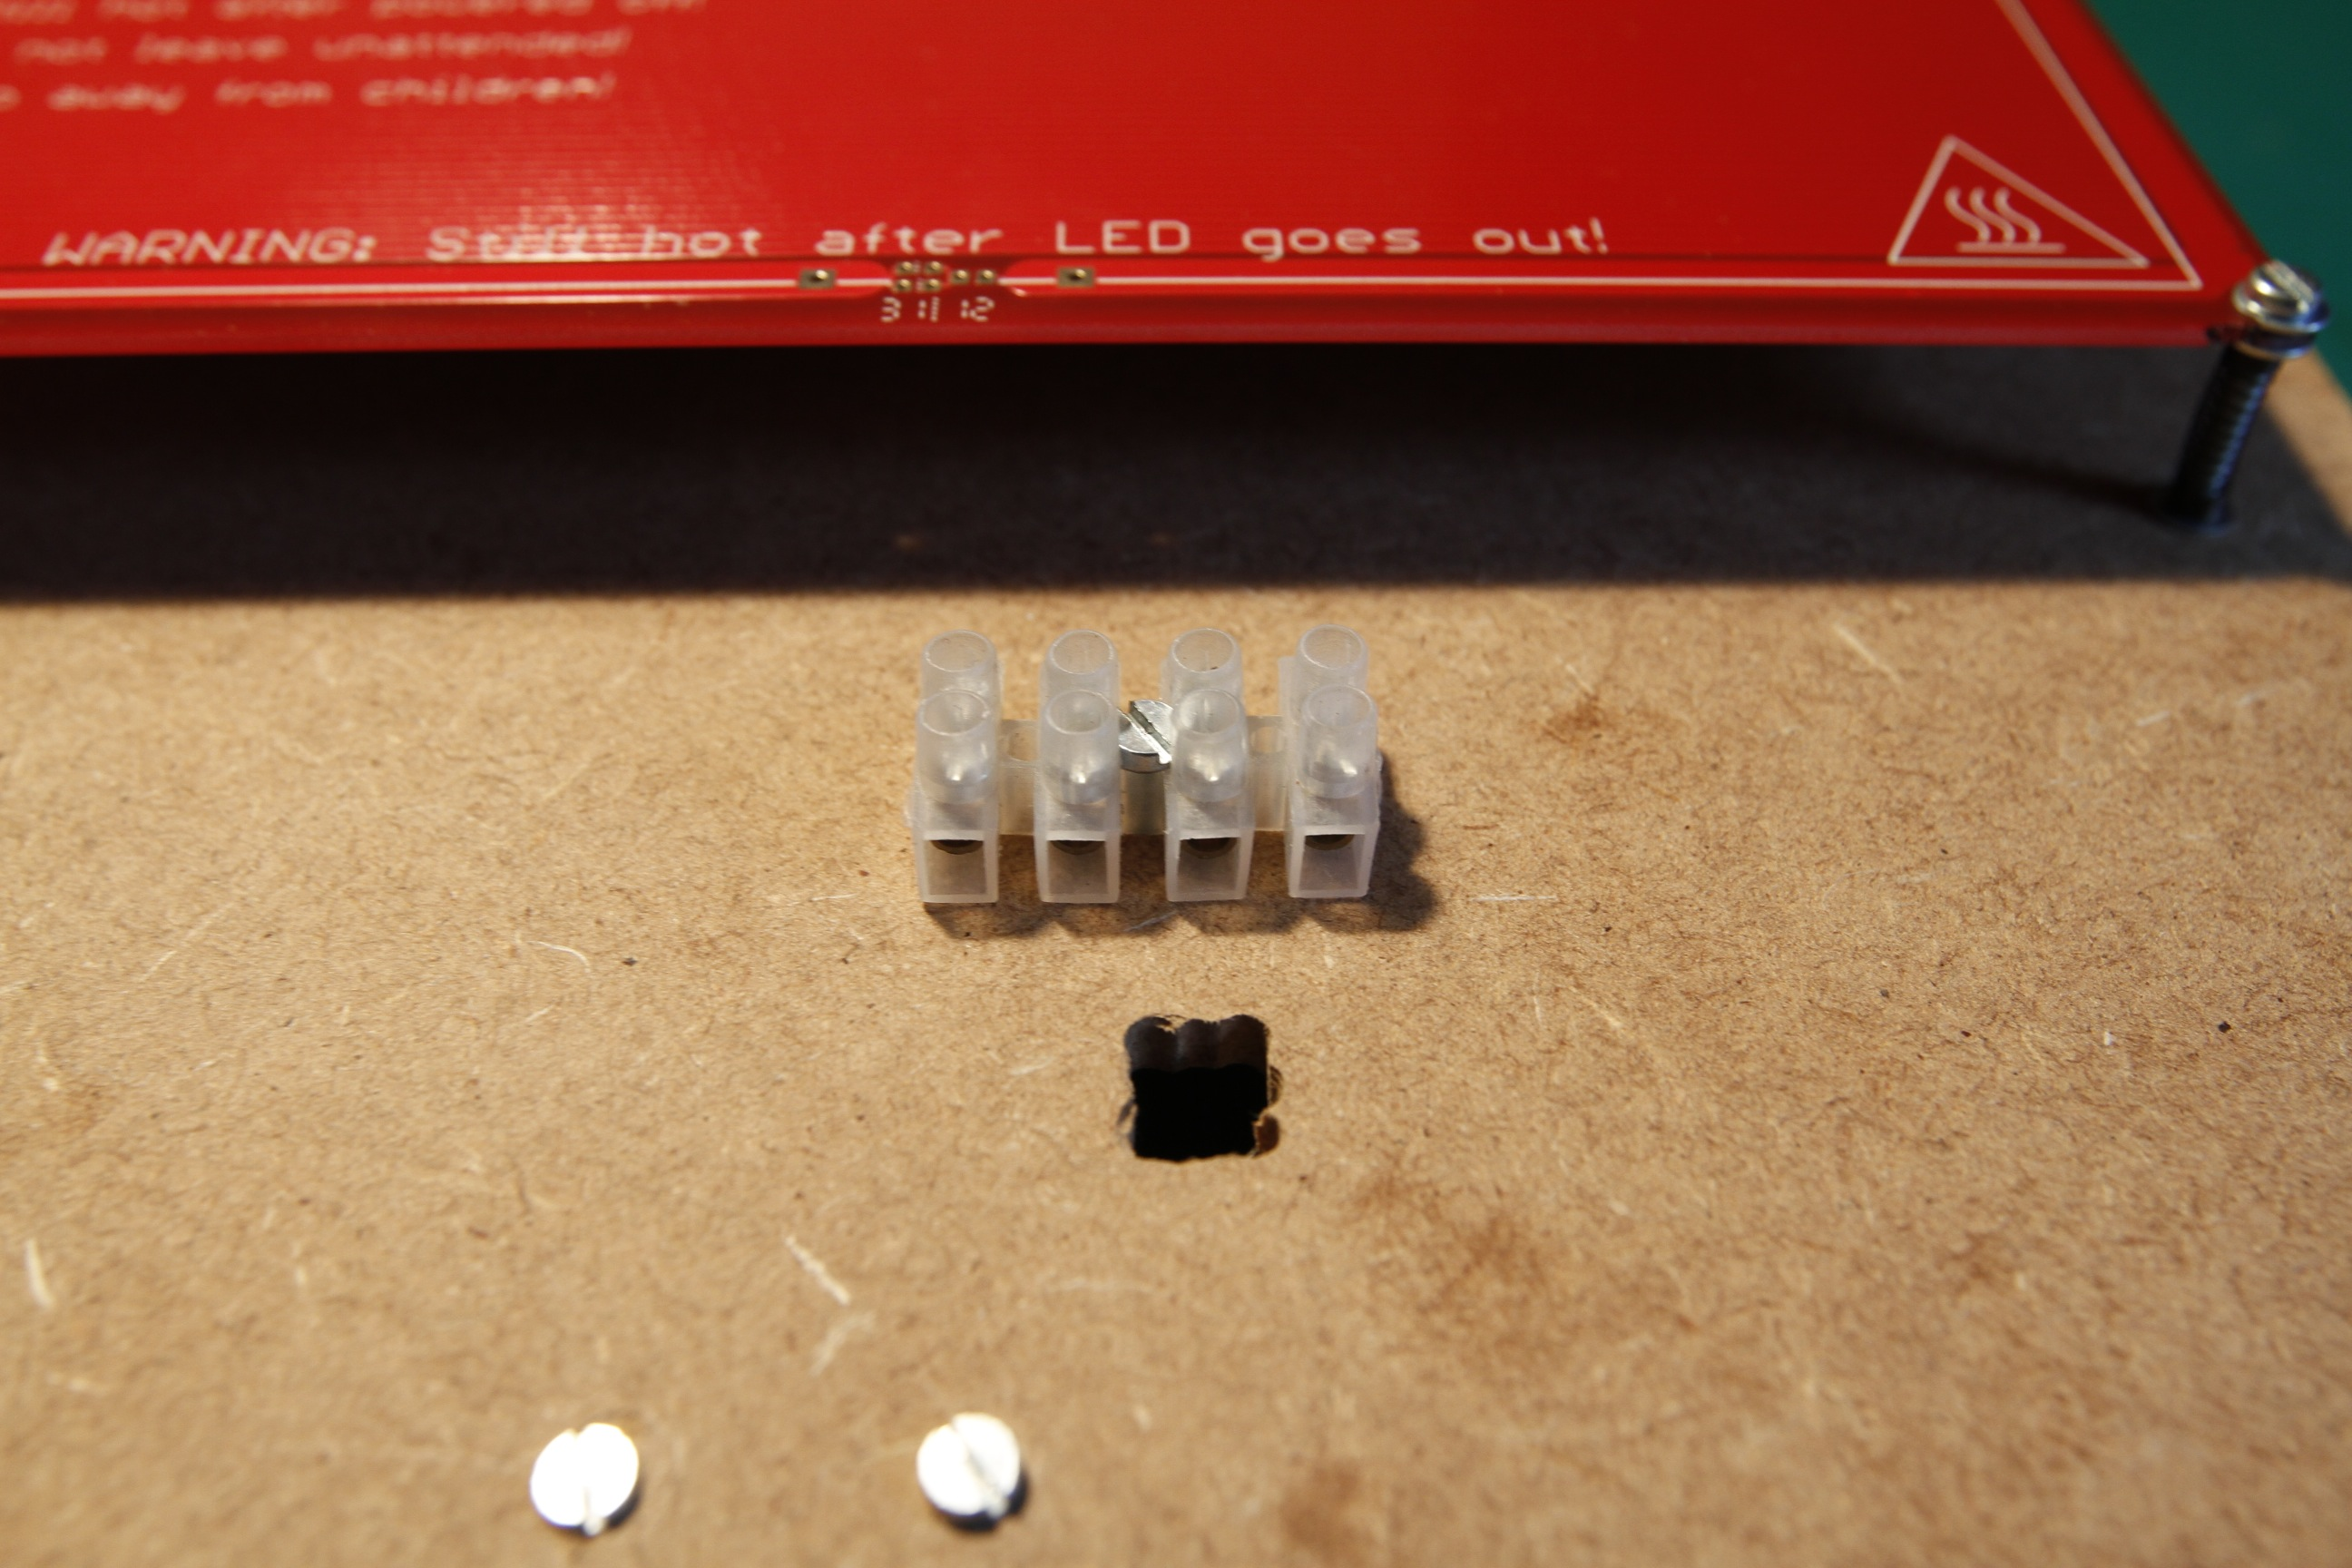
\includegraphics[width=0.7\textwidth]{../../Fotos/42.jpg}
			\caption{Posición de la clema}
			\label{fig:clema}
		\end{figure}
	El aspecto final de la tabla con todo montado lo podemos ver en la siguiente foto:
		\begin{figure}[H]
			\centering
			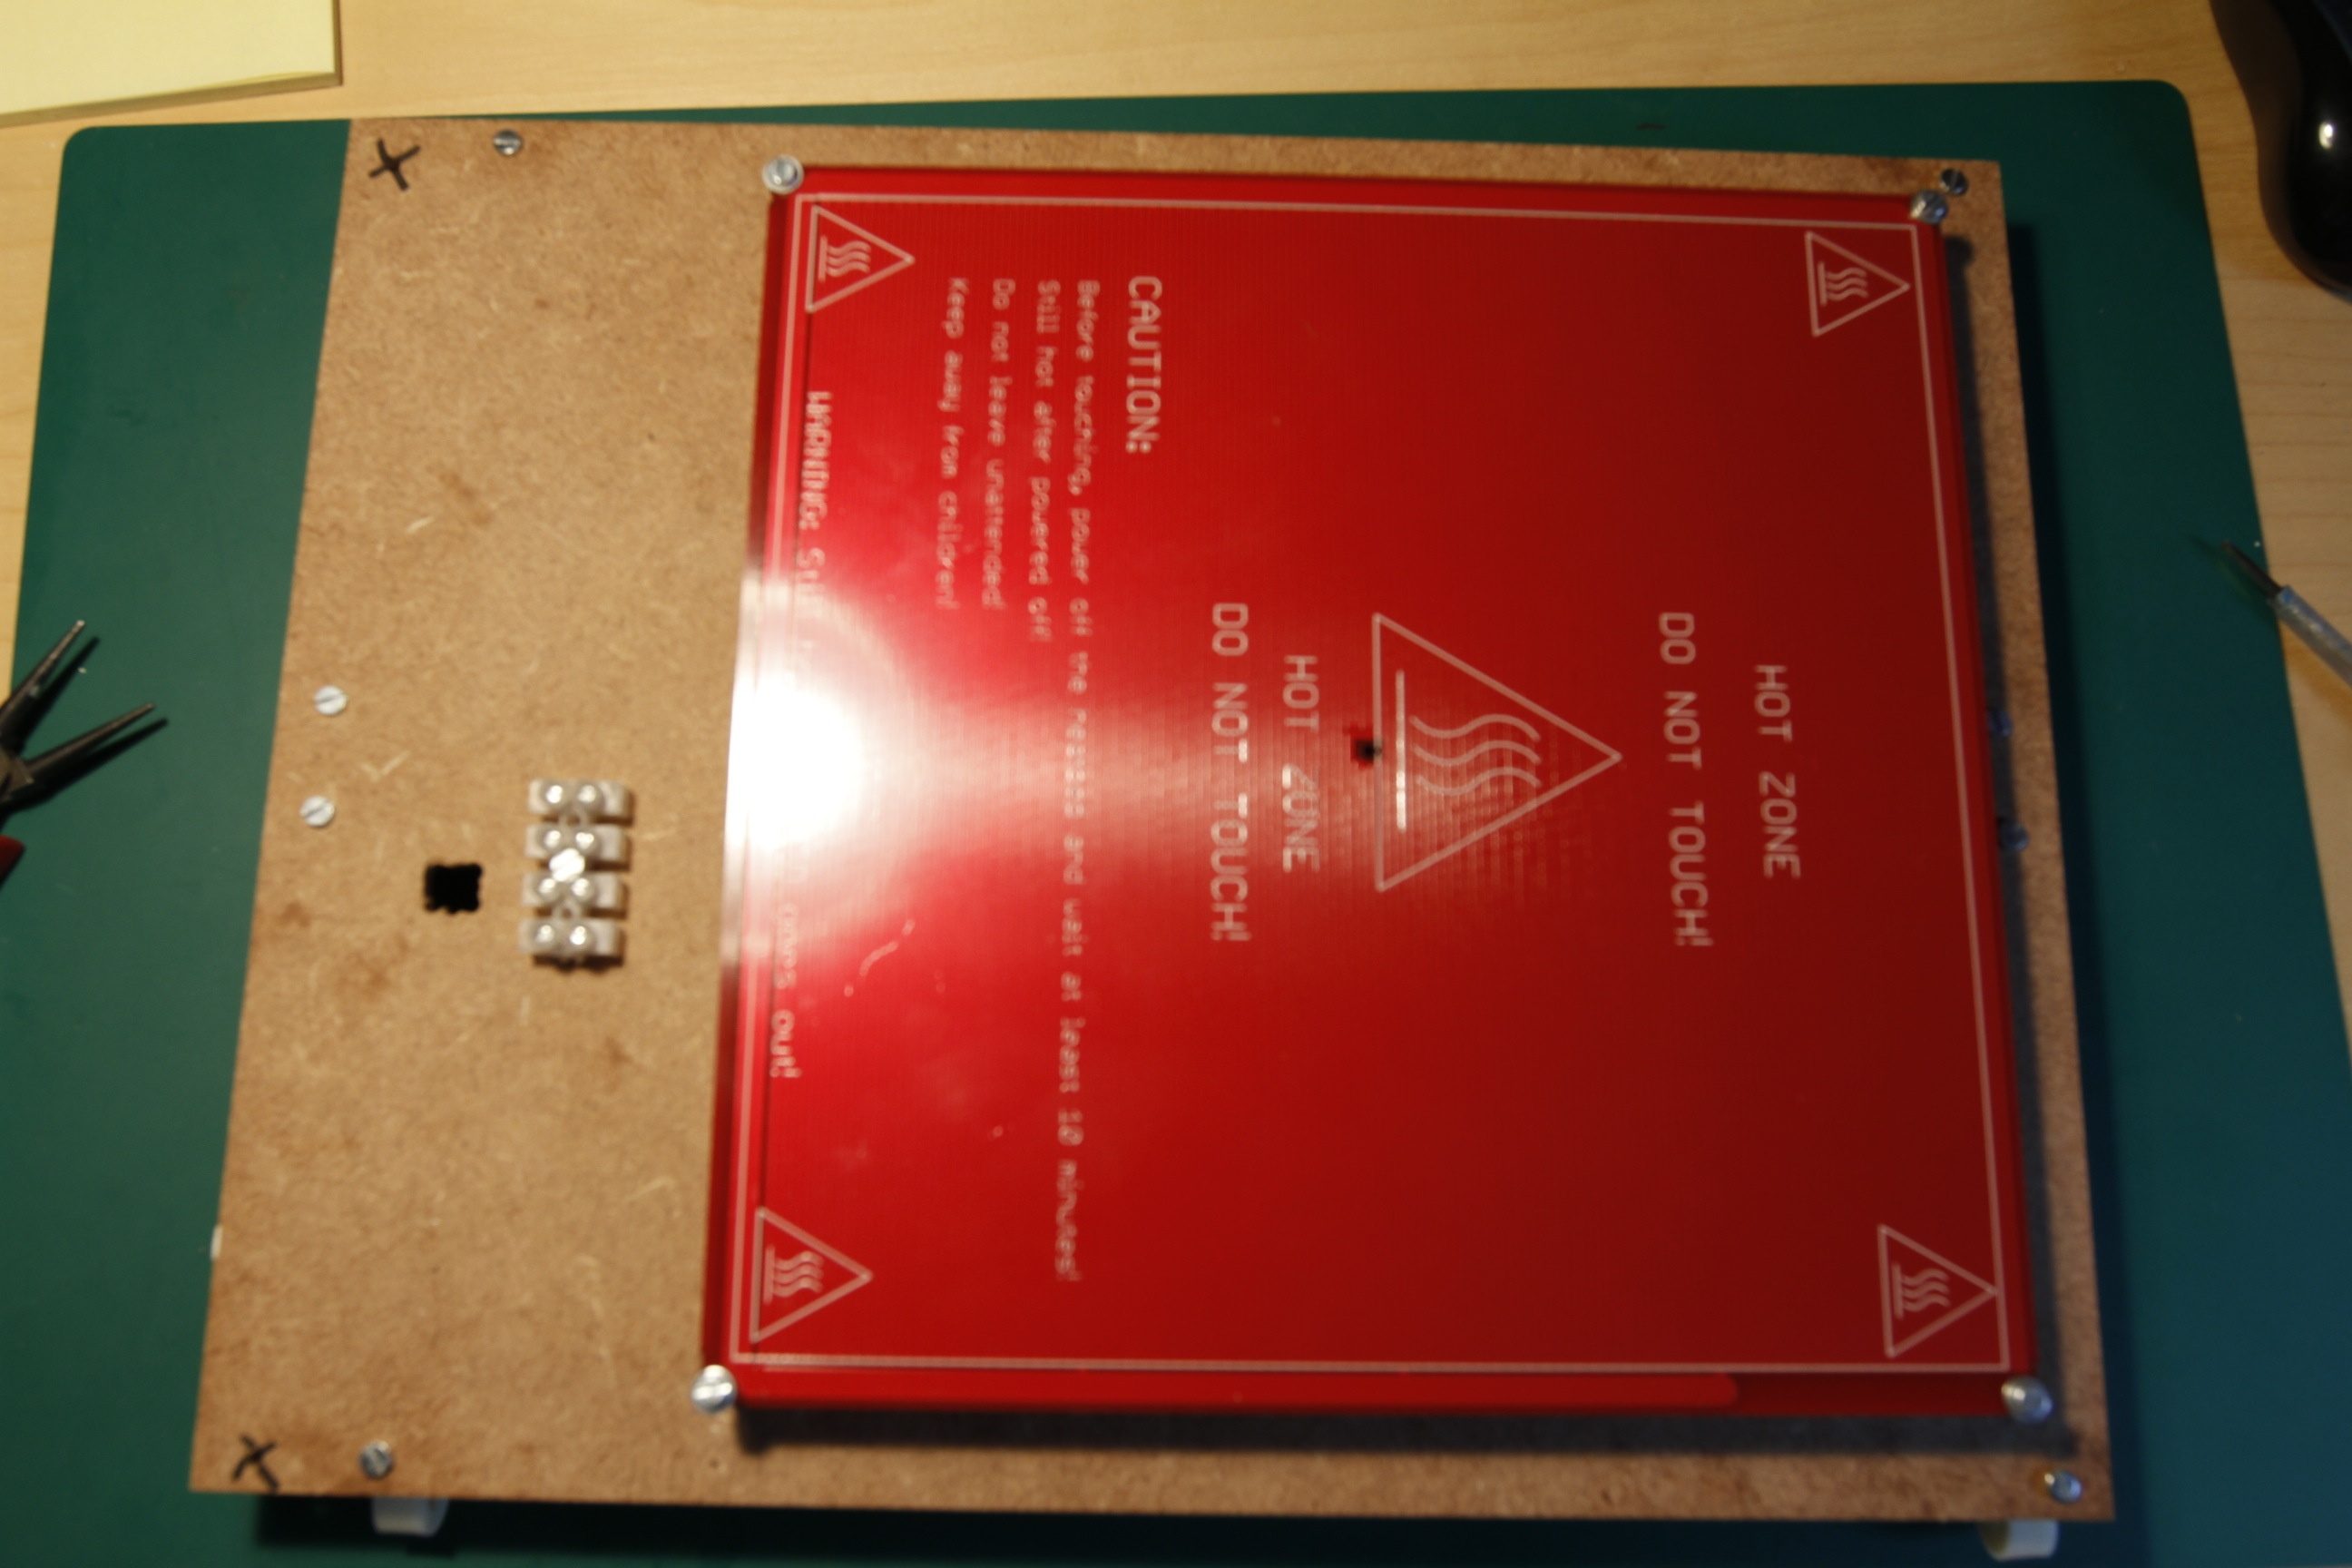
\includegraphics[width=0.7\textwidth]{../../Fotos/43.jpg}
			\caption{Eje Y terminado}
			\label{fig:eje.y}
		\end{figure}